% !TeX document-id = {9ad29ae0-fa76-4dc8-93c4-b92097f6aa60}
% !TeX TXS-program:compile = txs:///pdflatex/[--shell-escape]
\documentclass[landscape,a4paper]{article}
\usepackage[table]{xcolor}
\usepackage[normalem]{ulem}
\usepackage{tikz}
\usetikzlibrary{shapes,positioning,arrows,fit,calc,graphs,graphs.standard}
\usepackage[nosf]{kpfonts}
\usepackage[t1]{sourcesanspro}
\usepackage{multicol}
\usepackage{wrapfig}
\usepackage[top=0.5mm,bottom=1mm,left=1mm,right=1mm]{geometry}
\usepackage[framemethod=tikz]{mdframed}
\usepackage{microtype}
\usepackage{tabularx}
\usepackage{hhline}
\usepackage{makecell}
\usepackage{mathtools}
\usepackage{subfig}
\usepackage{listings}
\usepackage{soul}
\usepackage{amsmath,amsthm,amsfonts,amssymb}
\usepackage[font=tiny,labelfont=bf]{caption}
\usepackage[none]{hyphenat}
%\usepackage{minted}

\graphicspath{ {./imgs/} }

\DeclarePairedDelimiter{\ceil}{\lceil}{\rceil}

\definecolor{myblue}{cmyk}{1,.72,0,.38}

\pgfdeclarelayer{background}
\pgfsetlayers{background,main}

\renewcommand{\baselinestretch}{.8}
\pagestyle{empty}

\let\counterwithout\relax
\let\counterwithin\relax
\usepackage{chngcntr}
\usepackage{verbatim}
\usepackage{etoolbox}
\makeatletter
\preto{\@verbatim}{\topsep=0pt \partopsep=0pt }
\makeatother

\counterwithin*{equation}{section}
\counterwithin*{equation}{subsection}
\usepackage{enumitem}
\newlist{legal}{enumerate}{10}
\setlist[legal]{label*=\arabic*.,leftmargin=3mm}
\setlist[itemize]{leftmargin=3mm}
\setlist[enumerate, 1]{leftmargin=3.5mm}
\setlist{nosep}

\newenvironment{descitemize} % a mixture of description and itemize
{\begin{description}[leftmargin=*,before=\let\makelabel\descitemlabel]}
	{\end{description}}
\newcommand{\descitemlabel}[1]{%
	\textbullet\ \textbf{#1}%
}
\makeatletter

\renewcommand{\section}{\@startsection{section}{1}{0mm}%
	{.2ex}%
	{.2ex}%x
	{\color{myblue}\sffamily\scriptsize\bfseries}}
\renewcommand{\subsection}{\@startsection{subsection}{1}{0mm}%
	{.2ex}%
	{.2ex}%x
	{\sffamily\bfseries}}
\renewcommand{\subsubsection}{\@startsection{subsubsection}{1}{0mm}%
	{.2ex}%
	{.2ex}%x
	{\rmfamily\bfseries}}

\makeatother
\setlength{\parindent}{0pt}
\setlength\partopsep{-\topsep}

\newcolumntype{a}{>{\hsize=1.5\hsize}X}
\newcolumntype{b}{>{\hsize=.25\hsize}X}

\setlength\columnsep{10pt}
\setlength\columnseprule{0pt}
\begin{document}
	\abovedisplayskip=0pt
	\abovedisplayshortskip=0pt
	\belowdisplayskip=0pt
	\belowdisplayshortskip=0pt
%	\scriptsize
	\tiny
	\begin{multicols*}{4}
	\section{Model Evaluation}
	\subsection{Classification Metrics}
	\subsubsection{Accuracy}
	\[A=\frac{1}{m}\sum_{j=1}^{m}[\hat{y}_j=y_j]\]
	\begin{itemize}
		\item $\hat{y}_j$ is the predicted value
		\item $y_j$ is the ground truth value
		\item Interpreted as ratio of predicted elements that are equal to ground truth over total elements
		\item Accuracy other formula: $\frac{\text{TP+TN}}{\text{TP+TN+FP+FN}}$
	\end{itemize}
	\subsubsection{Confusion Matrix}
	\begin{center}
		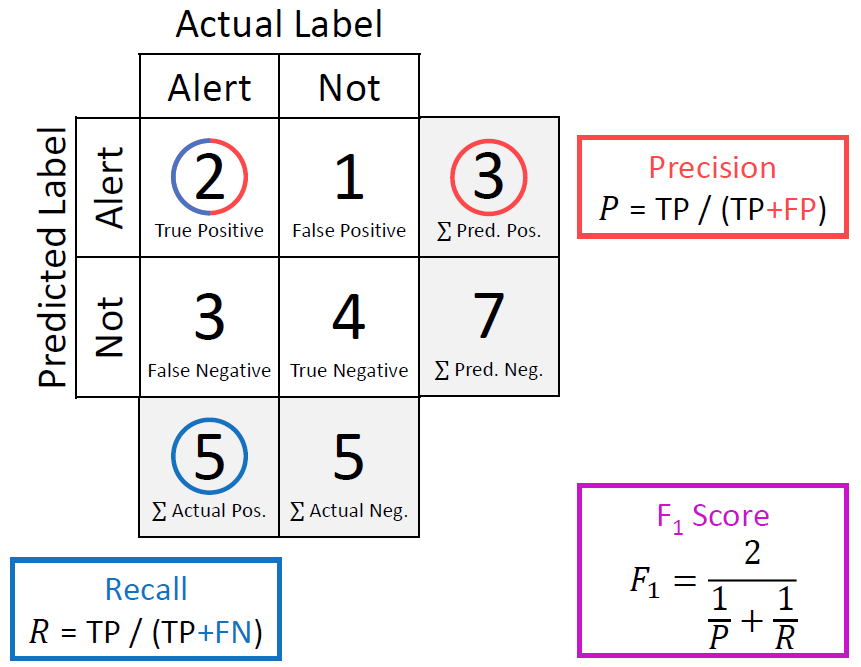
\includegraphics[width=0.5\columnwidth]{confusion-matrix}
	\end{center}
	\begin{itemize}
		\item Maximize \textbf{recall} to minimize \textbf{false negatives}
		\item Maximize \textbf{precision} to minimize \textbf{false positive}
		\item Only use F1 score if you cant justify between recall and precision
		\begin{itemize}
			\item F1 score is not just a simple average but is instead more robust as it is \textbf{less sensitive to extreme values}
		\end{itemize}
		\item Low metric score can be due to \textcolor{red}{imbalanced data}
	\end{itemize}
	\begin{center}
		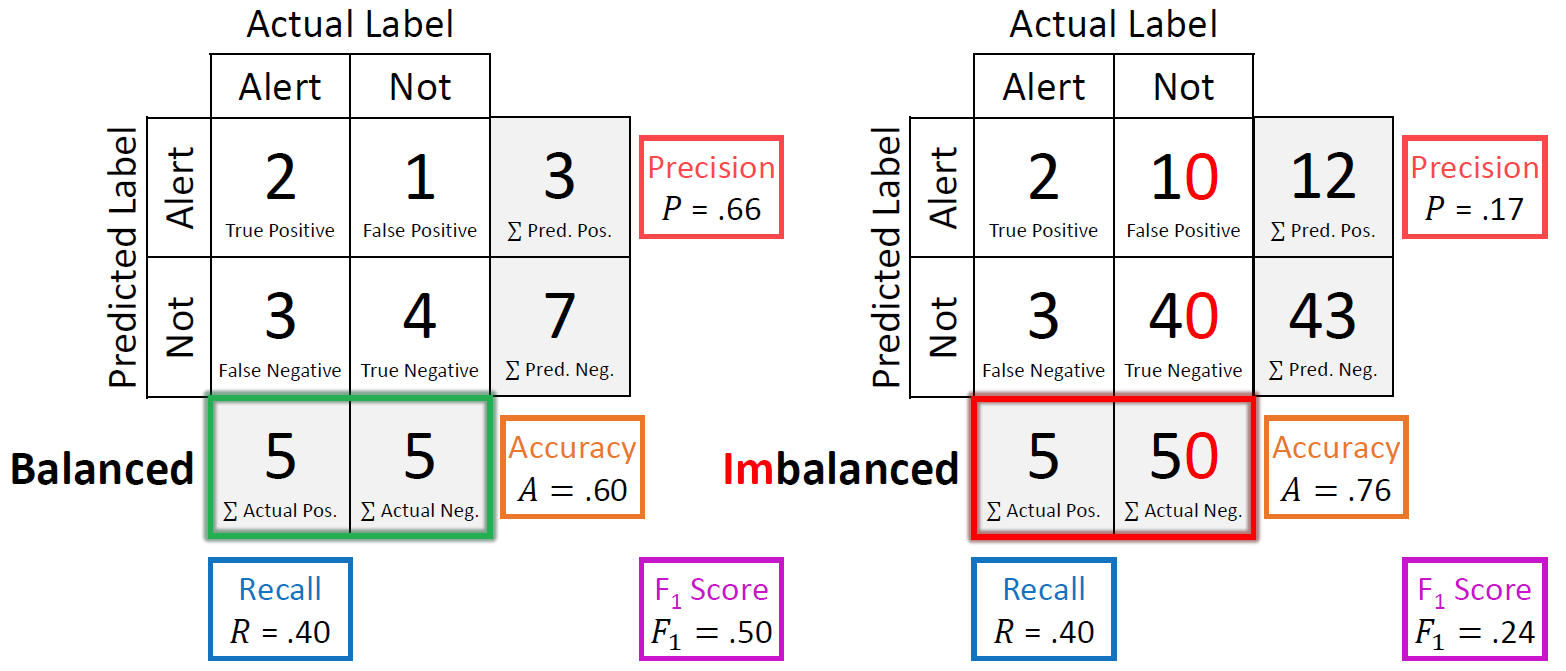
\includegraphics[width=0.5\columnwidth]{imbalanced}
	\end{center}
	\begin{itemize}
		\item Depends on \textbf{prediction threshold}
		\item If there is multiclass, we can use either \textbf{micro-average} or \textbf{macro-average}
		\begin{itemize}
			\item Micro-average weighs each \textbf{instance} equally and \textcolor{red}{accounts for imbalanced data}
			\item Macro-average weight each \textbf{class} equally and is used \textcolor{red}{only when real-world test data is balanced}
		\end{itemize}
	\end{itemize}
	\begin{tabular}{c c}
		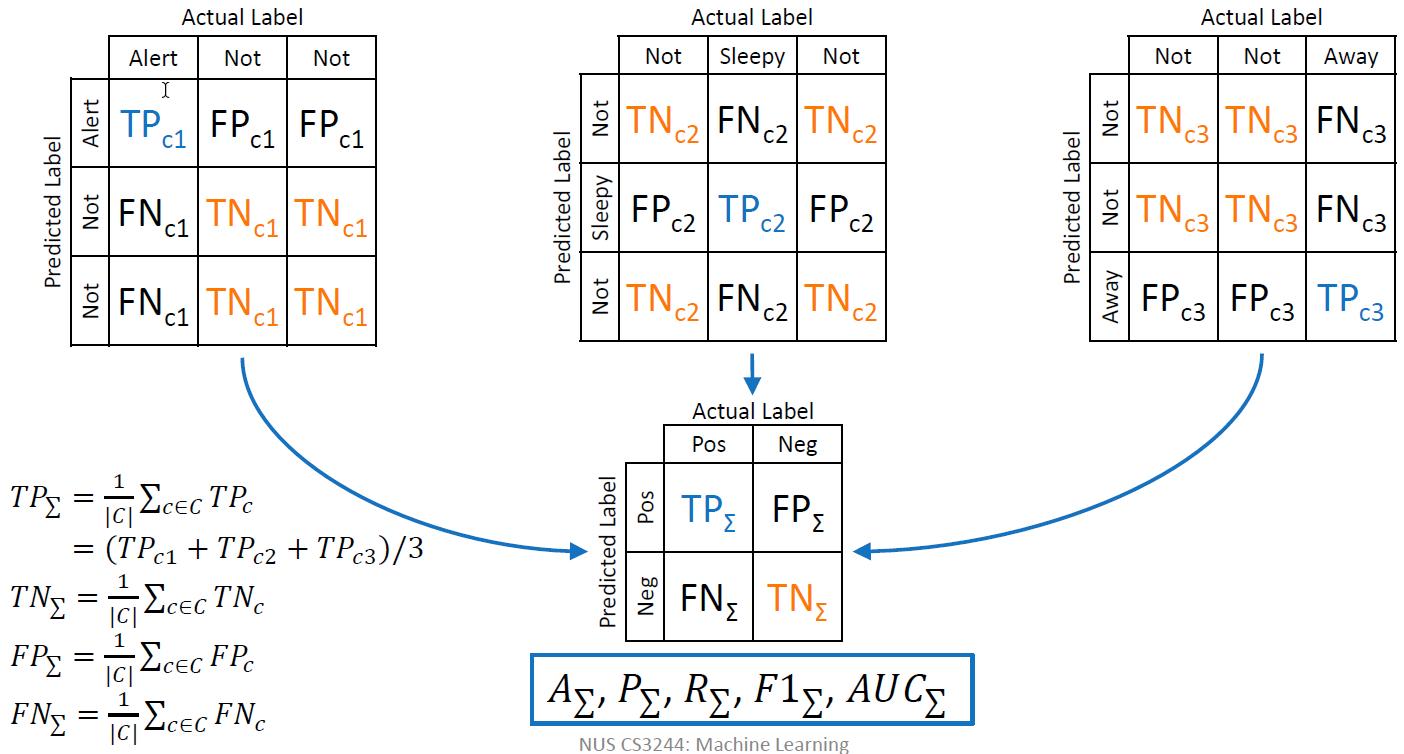
\includegraphics[width=0.45\linewidth]{micro-average}
		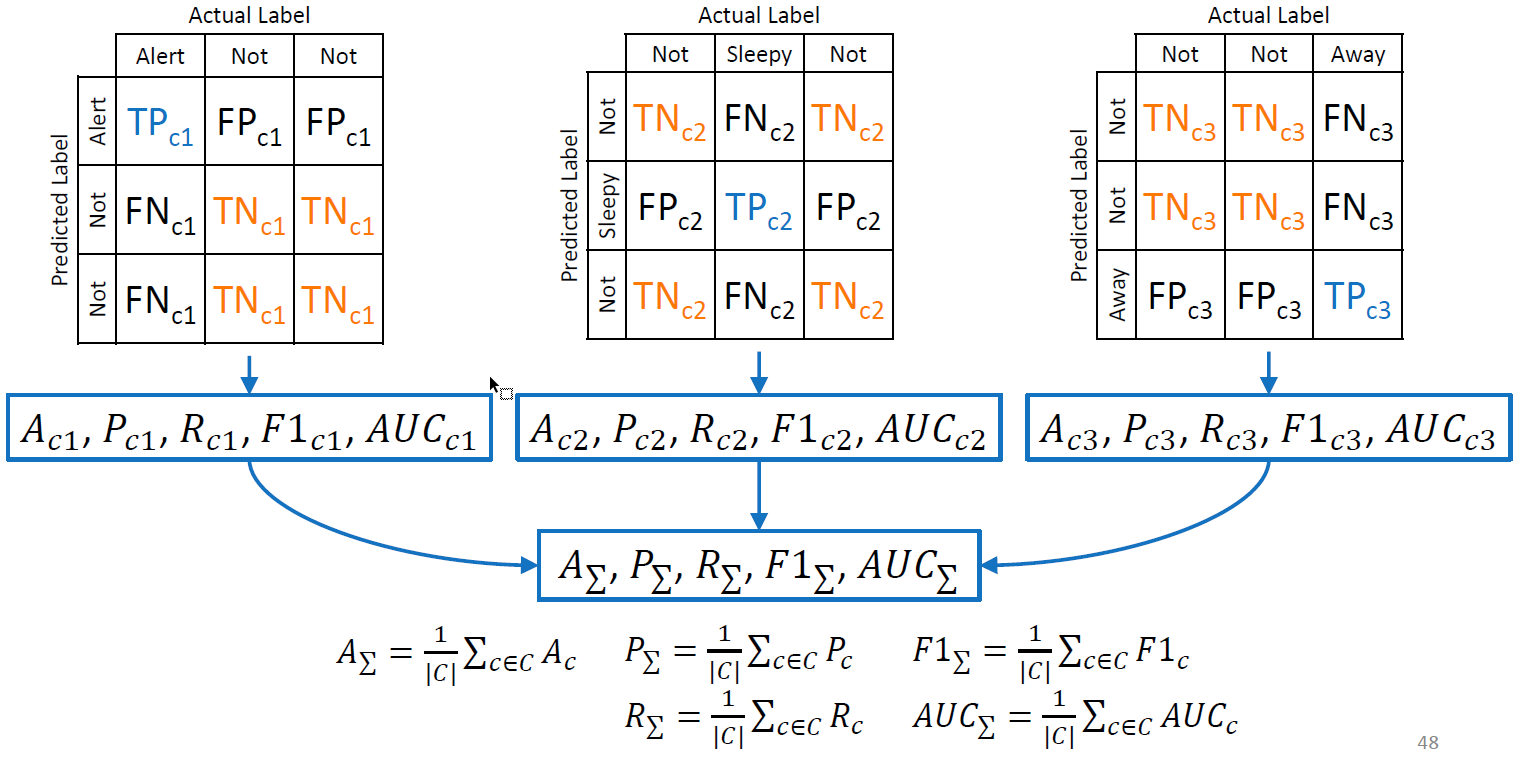
\includegraphics[width=0.55\linewidth]{macro-average}
	\end{tabular}
	\subsubsection{Receiver Operator Curve}
	\begin{center}
		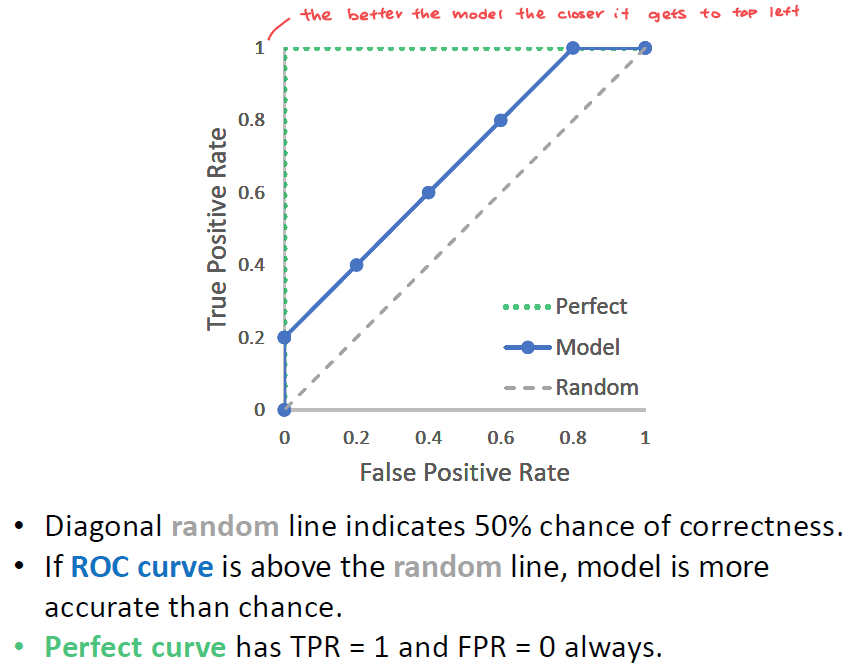
\includegraphics[width=0.5\columnwidth]{roc}
	\end{center}
	\subsubsection{Area Under Curve (AUC) of ROC}
	\begin{center}
		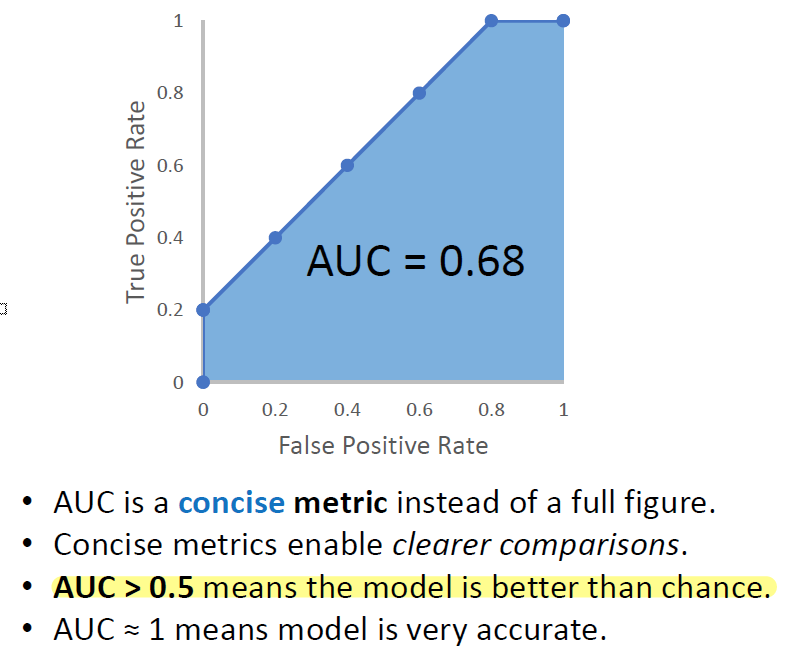
\includegraphics[width=0.5\columnwidth]{auc}
	\end{center}
	\subsection{Regression Evaluation Metrics}
	\subsubsection{Average Difference Metrics}
	\begin{center}
		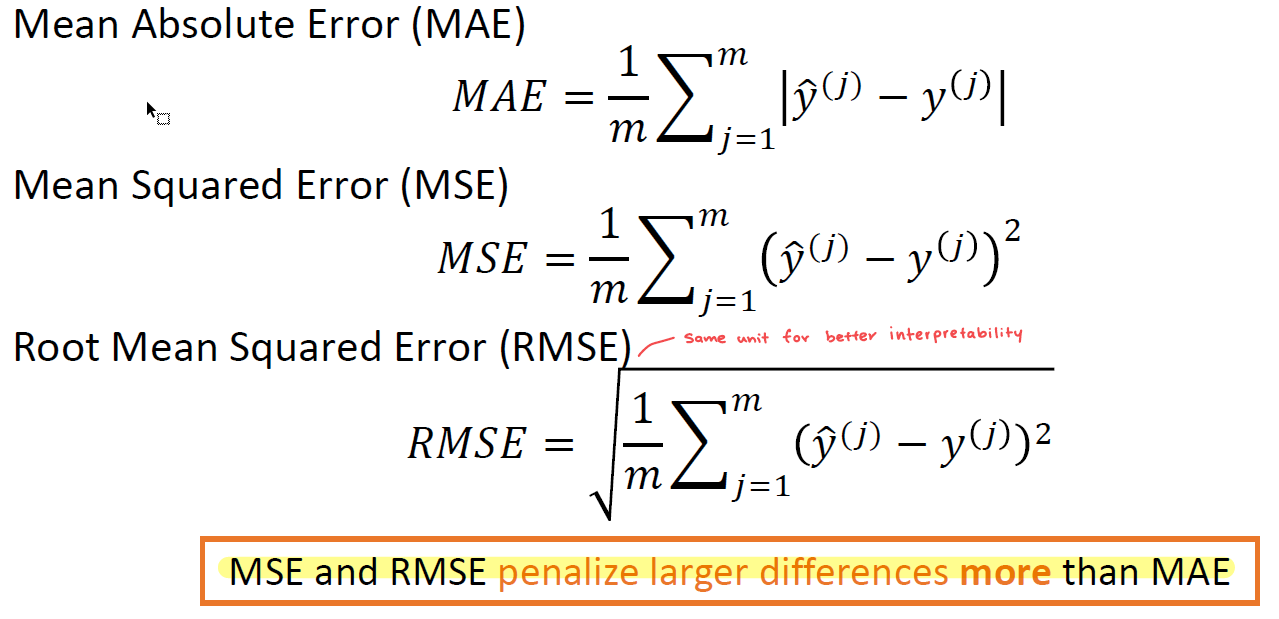
\includegraphics[width=0.55\columnwidth]{regression-metric}
	\end{center}
	\subsubsection{Vector Distances and Similarity}
	\begin{center}
		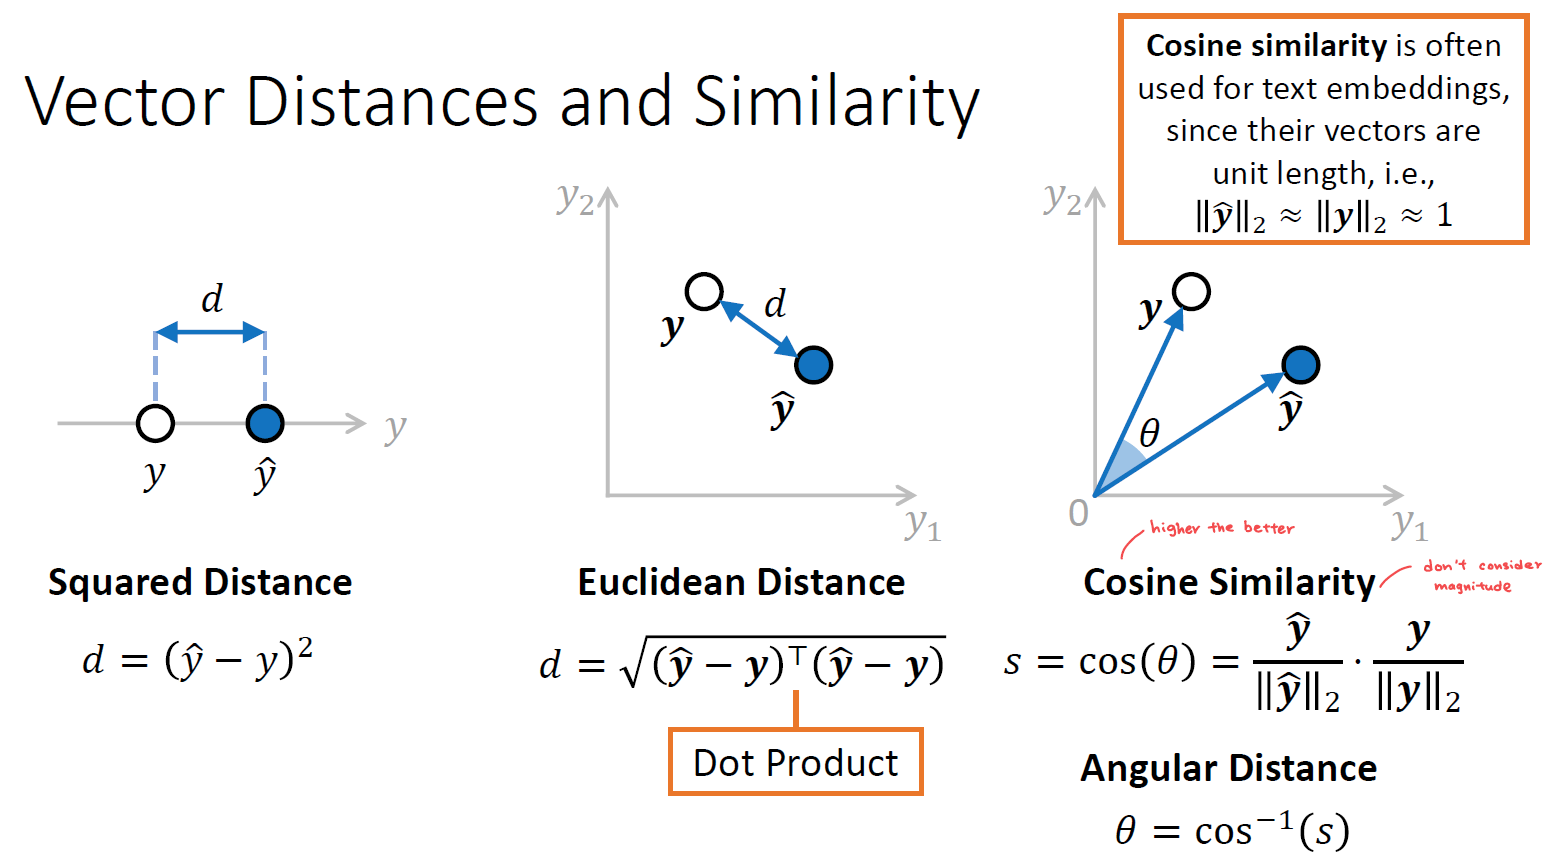
\includegraphics[width=0.55\columnwidth]{vector-metric}
	\end{center}
	\subsubsection{Difference between MSE and Euclidean Distance}
	\begin{itemize}
		\item MSE is the average of all the distances across the \textbf{test set} whereas euclidean distance is calculating the distance \textbf{across feature vector}
	\end{itemize}
	\begin{center}
		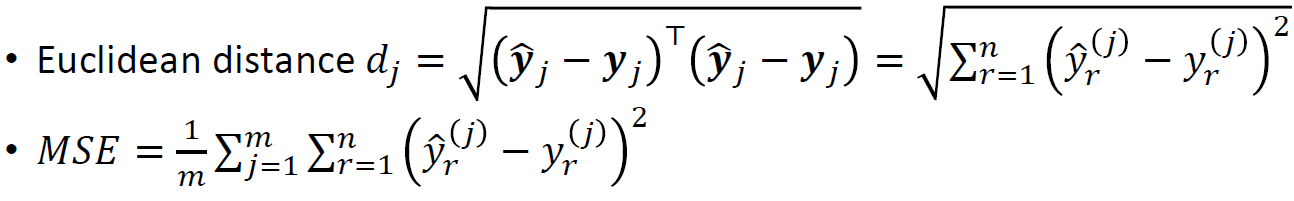
\includegraphics[width=0.5\columnwidth]{mse-vs-euclidean}
	\end{center}
	\section{Data Processing}
	\subsection{Linear Separability}
	\begin{itemize}
		\item In most real-world scenario, \textbf{data tends to not be linearly separable} (e.g. images, time-series data, text). Wrongly assuming that data features are linearly separable leads to irrelevant features being \textbf{uninformative} to train the model to discriminate
		between prediction labels
		\item Check using \textbf{scatterplot} (if only 2 features) and \textbf{scatterplot matrix} (if more than 2 features). We can also obtain a computational metric using \textbf{linear SVM}
	\end{itemize}
	\subsubsection{Testing Liner Separability using Linear SVM}
	\begin{center}
		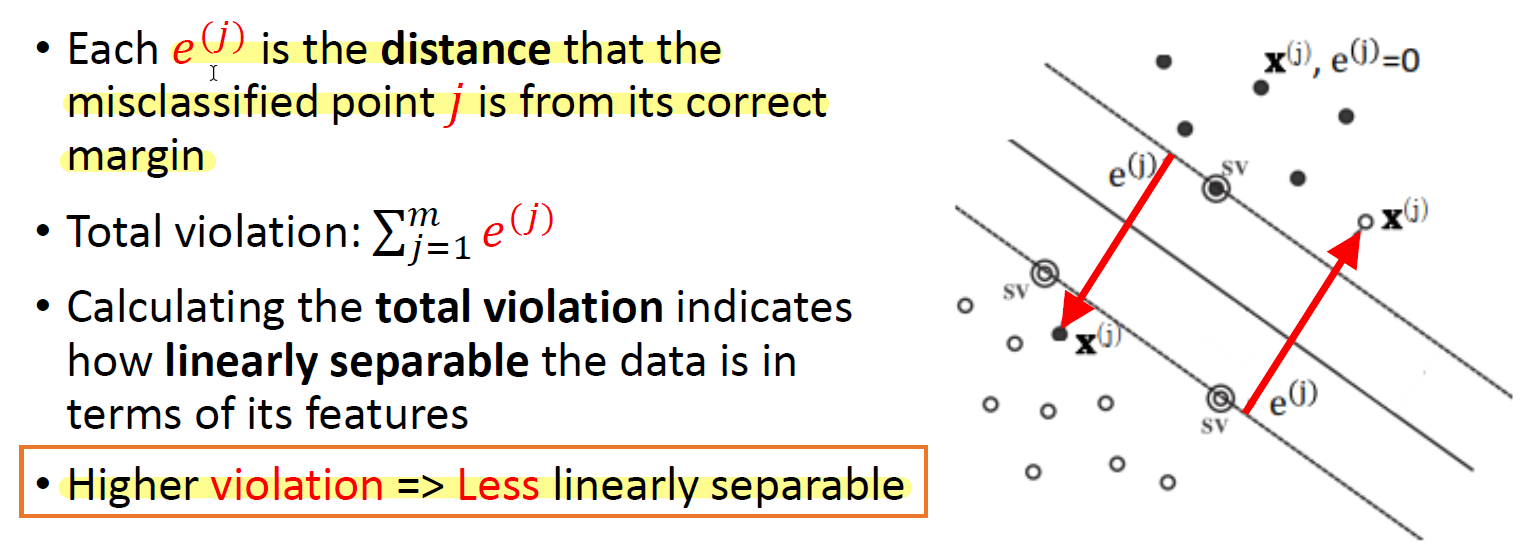
\includegraphics[width=0.6\columnwidth]{linear-separability-svm}
	\end{center}
	\subsubsection{Mitigation}
	\begin{enumerate}
		\item Find useful features through feature extraction (collecting new features)
		\item Transform features
		\begin{itemize}
			\item Feature engineering ($x\rightarrow x^2$)
			\item Change Basis Vectors (PCA, LDA)
			\item Kernel trick
			\item Features Learning (Neural Network)
		\end{itemize}
	\end{enumerate}
	\subsubsection{Principal Component Analysis (PCA)}
	\begin{itemize}
		\item PCA uses orthogonal transformation to convert a set of observations into a set of values of linearly uncorrelated variables called principal components
		\item Each principle component is a mix of features (e.g. PC1 can be 4 parts $x_1$, 1 part $x_2$)
		\item We can then plot out something called a scree graph which tells you which Principle components are important and we can just keep those to \textbf{reduce dimensionality}
		\item \textcolor{red}{Higher variance means more information}
		\item \textbf{Feature Normalization} needs to be done
	\end{itemize}
	\subsubsection{Linear Discriminant Analysis (LDA)}
	\begin{itemize}
		\item LDA works by projecting the data onto a lower-dimensional space that maximizes the separation between the classes
		\item Uses the F-test metrics: $F=\frac{|\mu_r-\mu_b|^2}{s_r^2+s_b^2}$
		\item The F-test scores are tied to each linear discriminant and the \textbf{higher F-test score means it separates classes better}
		\item Discard LD with low F-test to reduce dimensions
	\end{itemize}
	\subsubsection{PCA vs LDA}
	\begin{center}
		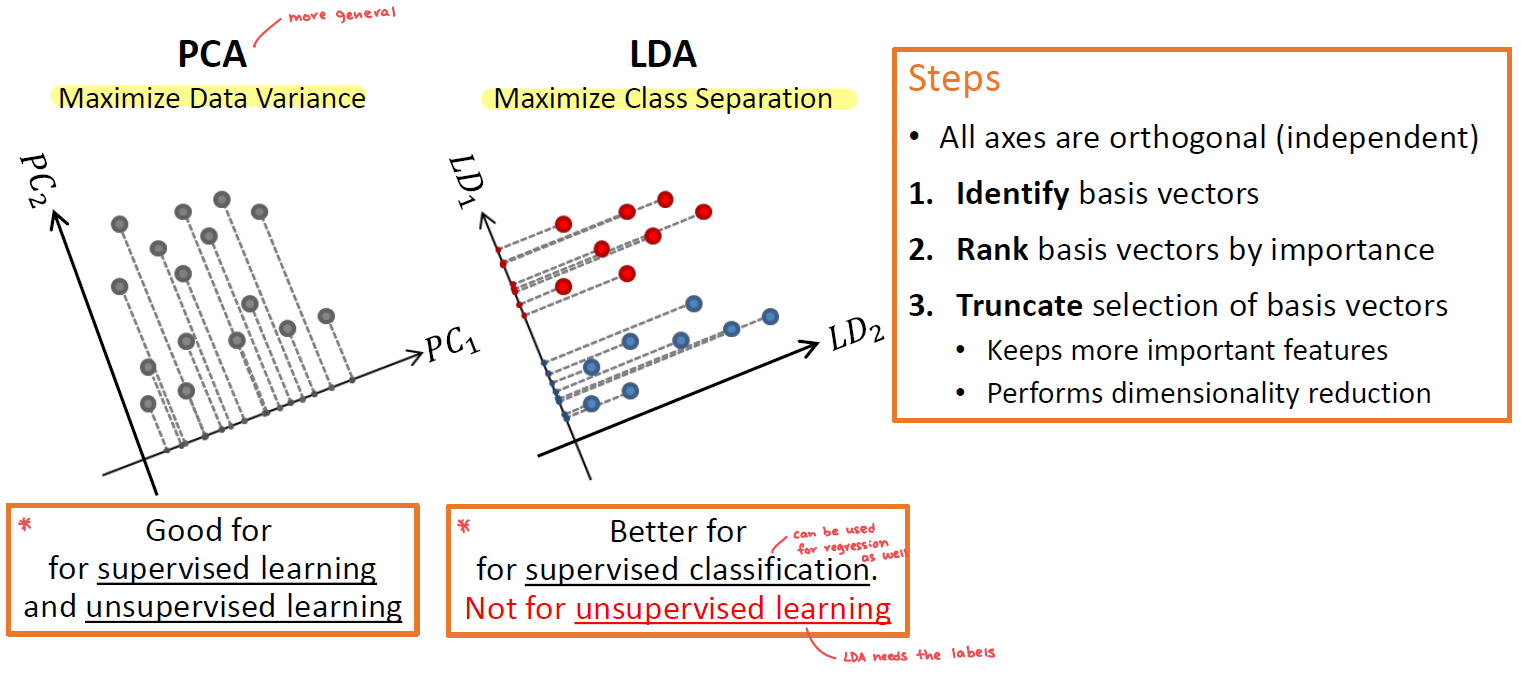
\includegraphics[width=0.6\columnwidth]{pca-vs-lda}
	\end{center}
	\subsection{Curse of Dimensionality}
	\begin{itemize}
		\item Curse of dimensionality occurs when there are way more features than data points ($n\gtrsim m$) are if we are dealing with unstructured data (e.g. images, sensor data)
		\item Causes problems like \textbf{overfitting} since data are too sparse to inform about true decision boundary and model can easily fit to sparse data
		\item Also a problem for clustering (e.g. knn) since distance are too similar
		\item Check using histogram of distances (check for \textbf{variance})
		\begin{itemize}
			\item Generally tedious to check various, general rule of thumb is for features to be $\frac{1}{5}$ of data points
		\end{itemize}
	\end{itemize}
	\subsubsection{Migrations}
	\begin{itemize}
		\item Feature selection
		\begin{itemize}
			\item Wrapper method (e.g. Recursive Feature Elimination, \textbf{Elbow method})
			\item Filter method (e.g. Only keep high info gain features, remove correlated features)
		\end{itemize}
		\item Dimensionality Reduction
		\begin{itemize}
			\item Linear Matrix Factorization: PCA, LDA
			\item Auto Encoders
			\item Feature Selection helps to enable \textbf{faster model training} and \textbf{better intepretability}
		\end{itemize}
	\end{itemize}
	\subsection{Imbalanced Data}
	\begin{itemize}
		\item Values not evenly distributed in features due to rare events (e.g. rare cancer) or skewed data collection
		\item Leads to evaluation metrics being \textbf{misleading} to interpret and models \textbf{overfitting} to majority class
		\item Can be checked easily by using histogram or bar chart of features
	\end{itemize}
	\columnbreak
	\subsubsection{Mitigation}
	\begin{itemize}
		\item Collect more data instance
		\item Resample instances (undersampling, oversampling, SMOTE)
		\item Undersampling should only be used when there is not much loss of data (e.g. 55\% majority class VS 45\% minority class)
		\item If data is very largely imbalanced, then oversampling/SMOTE is preferred so that we don't lose too much data
	\end{itemize}
	\begin{tabular}{c c}
		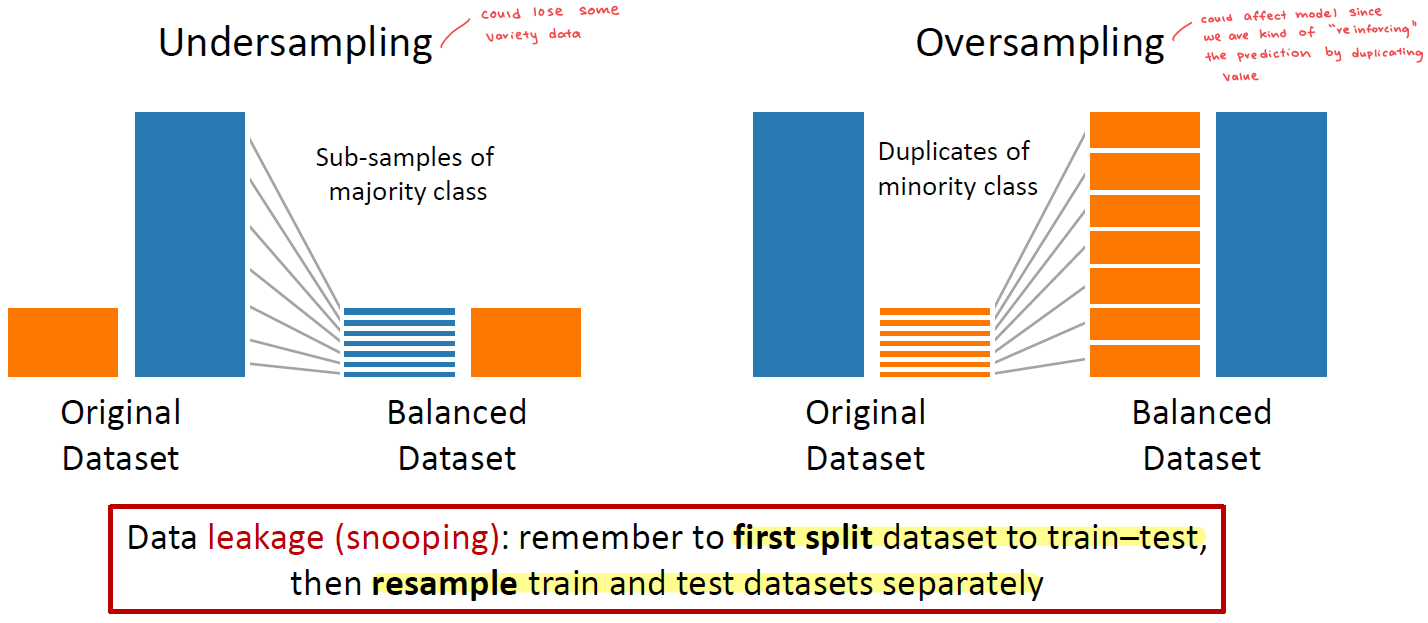
\includegraphics[width=0.5\linewidth]{data-resampling}
		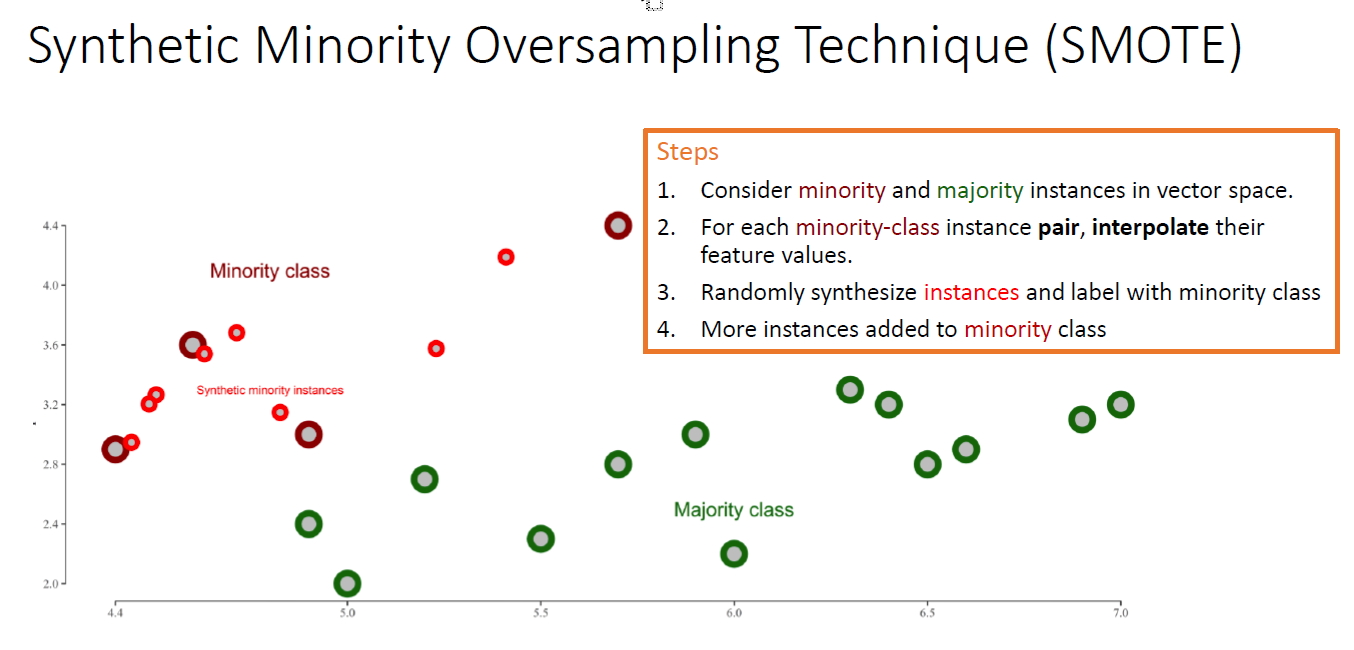
\includegraphics[width=0.5\linewidth]{smote}
	\end{tabular}
	\section{Feature Engineering}
	\subsection{Feature Extraction and Engineering}
	\begin{itemize}
		\item Process of \textbf{transforming raw data} to improve the accuracy of models
		\item Benefits:
		\begin{itemize}
			\item \textbf{Capture domain knowledge} (e.g., periodicity or relationships between
			features)
			\item \textbf{Express non-linear relationships} using linear models
			\item \textbf{Encode non-numeric features} to be used as inputs to models
		\end{itemize}
	\end{itemize}
	\begin{center}
		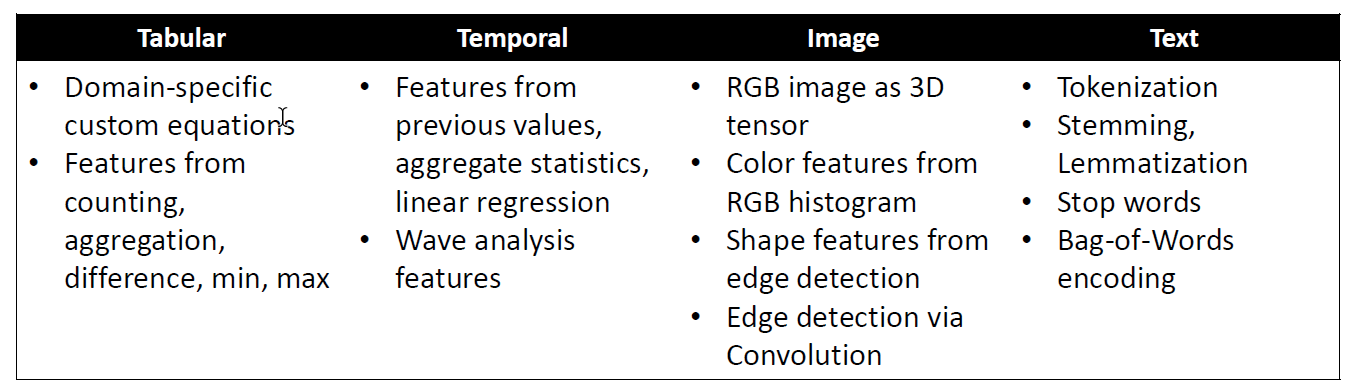
\includegraphics[width=0.7\columnwidth]{feature-engineering}
	\end{center}
	\section{Perceptron \& Neural Networks}
	\subsection{Perceptron Classification}
	\begin{center}
		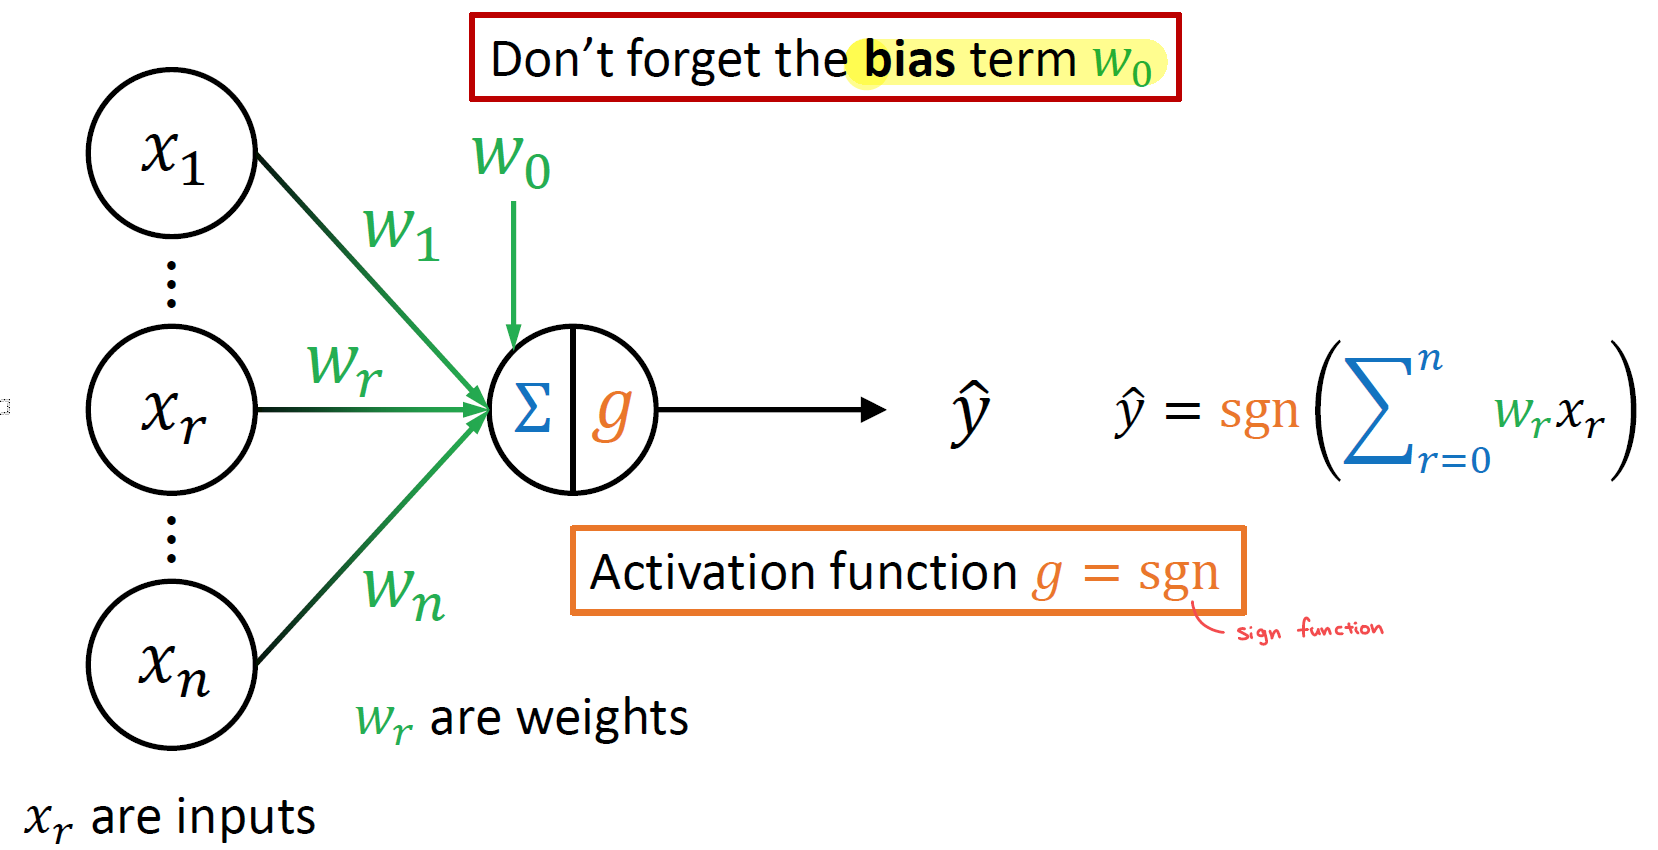
\includegraphics[width=0.6\columnwidth]{perceptron-classification}
	\end{center}
	\begin{itemize}
		\item Takes in a vector of input which are assigned \textbf{weights}
		\item Prediction class $\hat{y}$ is given by applying the \textbf{activation function} $g$ on the summation of the individual inputs multiplied by their weights$\rightarrow\hat{y}=g(w\cdot x)=g(w^Tx)$
	\end{itemize}
	\subsection{Perceptron Learning Algorithm (PLA)}
	\begin{itemize}
		\item One of the simplest way to learn what weights to assign to inputs and is \textbf{typically not used} in modern ML approach. \textcolor{red}{Never converges for non-linear or noisy data}
	\end{itemize}
	\begin{center}
		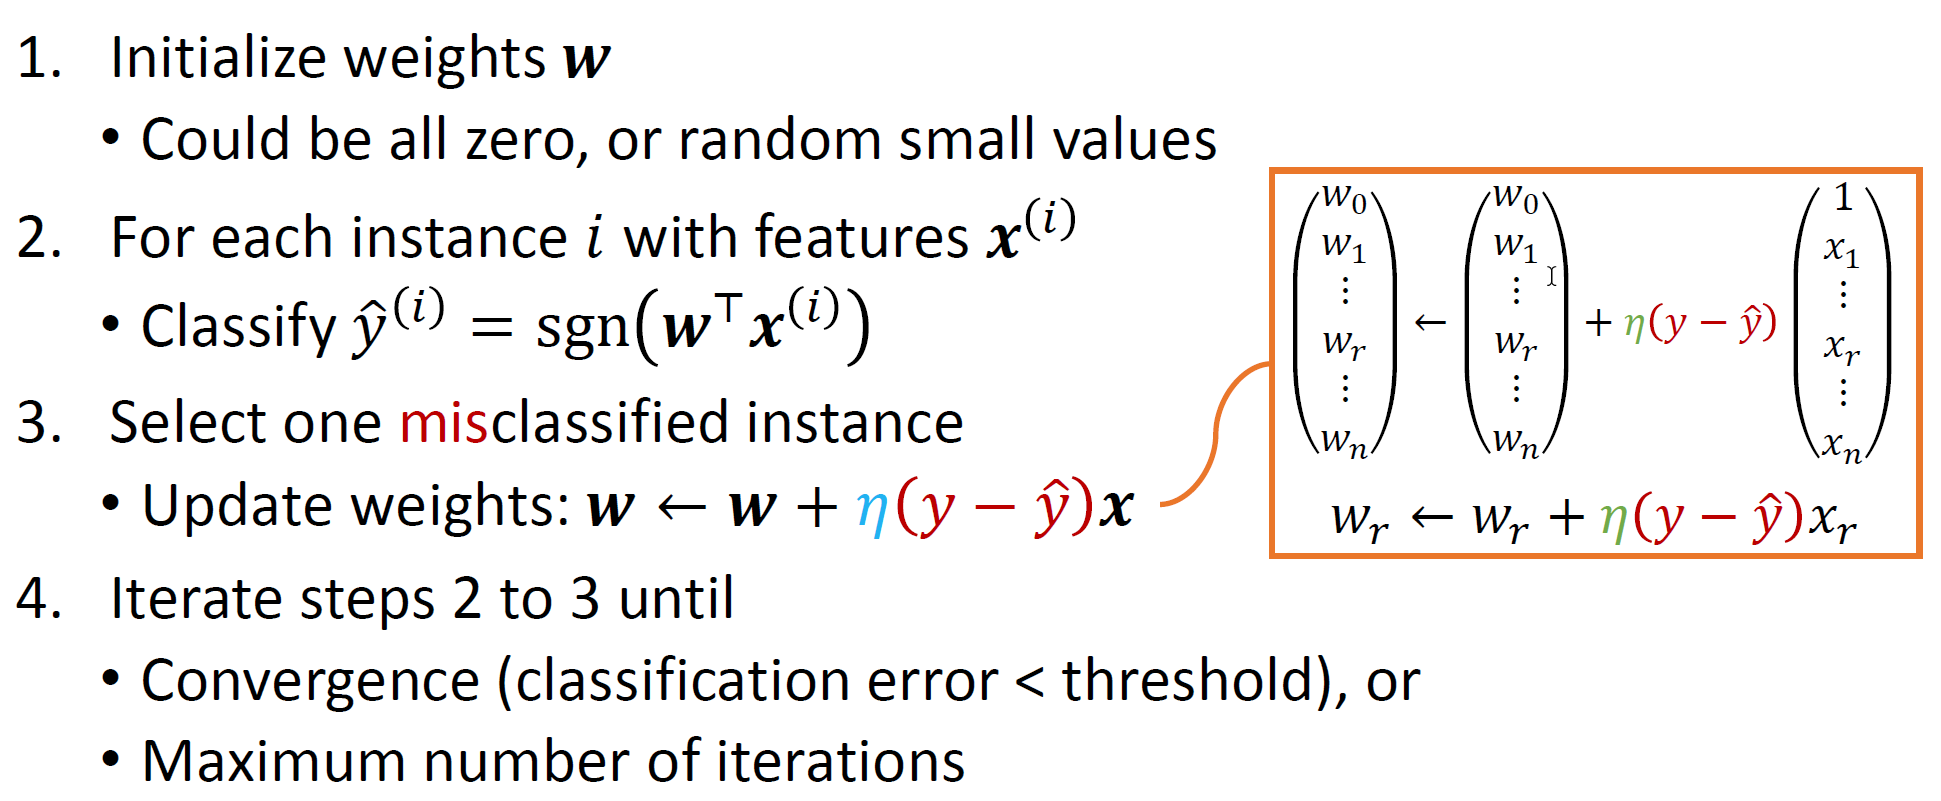
\includegraphics[width=0.7\columnwidth]{pla}
	\end{center}
	\begin{itemize}
		\item The update of weight is given by $w\leftarrow w+\eta (y-\hat{y})x$, where LHS $w$ is the new weight, RHS $w$ is the old weight, $\eta$ is the learning rate and $(y-\hat{y})$ is the learning error
	\end{itemize}
	\begin{center}
		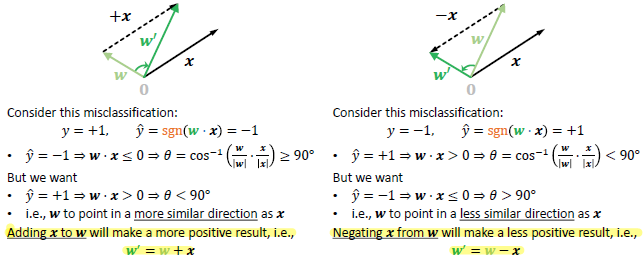
\includegraphics[width=0.7\columnwidth]{perceptron-weight-update}
	\end{center}
	\begin{itemize}
		\item Metric used to measure learning error is \textbf{cosine similarity}
	\end{itemize}
	\begin{center}
		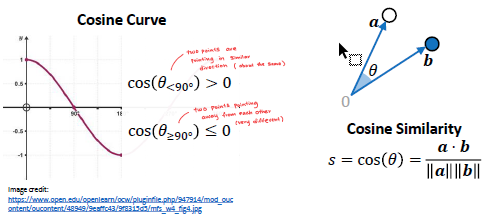
\includegraphics[width=0.7\columnwidth]{consine-similarity}
	\end{center}
	\subsection{Perceptron vs Linear SVM}
	\begin{center}
		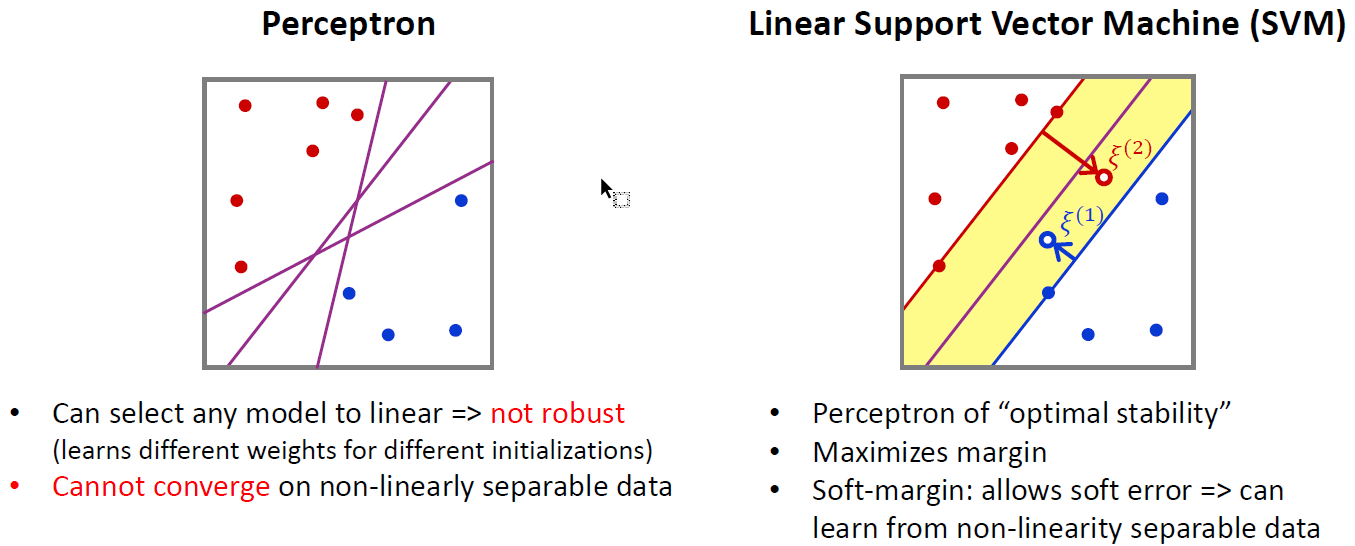
\includegraphics[width=0.7\columnwidth]{perceptron-vs-svm}
	\end{center}
	\subsection{Activation Functions}
	\begin{minipage}{0.3\columnwidth}
		\begin{center}
			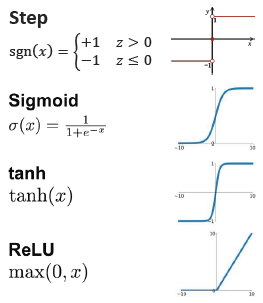
\includegraphics[width=1\columnwidth]{activation-functions}
		\end{center}
	\end{minipage}
	\begin{minipage}{0.7\columnwidth}
		\begin{itemize}
			\item 4 common activation functions are sign, sigmoid, tanh and ReLU
			\item All 4 activation functions are \textbf{differentiable}, allowing for gradient descent to be used to find minimum of error faster
			\item Sigmoid, tanh and ReLU are non-linear functions which allows for models to introduce \textbf{non-linearity} and create a non-linear, more complex decision boundary
		\end{itemize}
	\end{minipage}
	\subsection{Gradient Descent}
	\begin{center}
		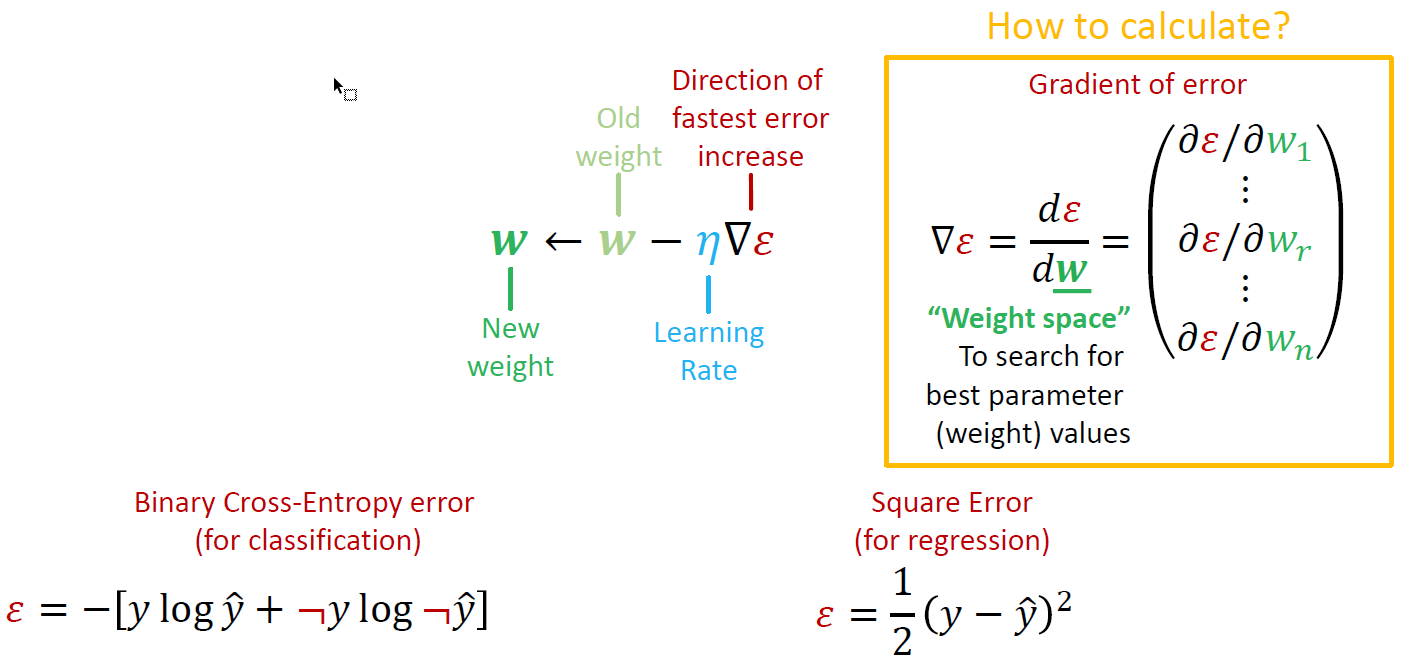
\includegraphics[width=0.7\columnwidth]{gradient-descent}
	\end{center}
	\subsubsection{Gradient of Error}
	\begin{itemize}
		\item Uses chain rule to determine the gradient/derivative of error
	\end{itemize}
	\begin{center}
		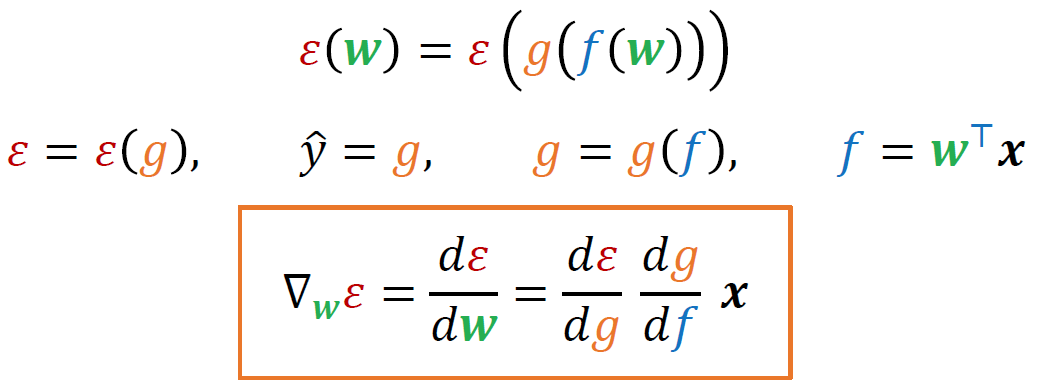
\includegraphics[width=0.5\columnwidth]{gradient-chain-rule}
	\end{center}
	\subsubsection{Summary of Gradient Calculation for Activation Functions}
	\begin{center}
		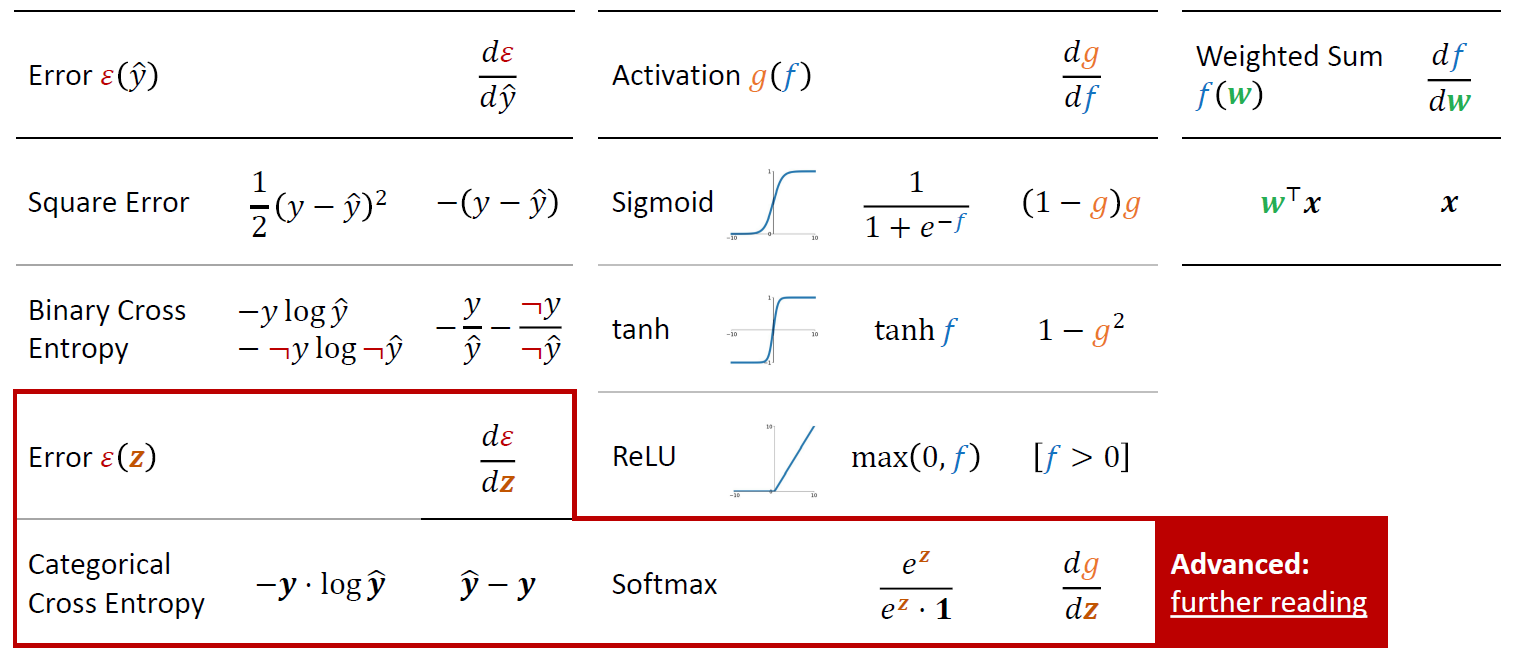
\includegraphics[width=0.7\columnwidth]{gradient-summary}
	\end{center}
	\subsection{Artificial Neural Network (ANN)}
	\begin{tabular}{c c}
		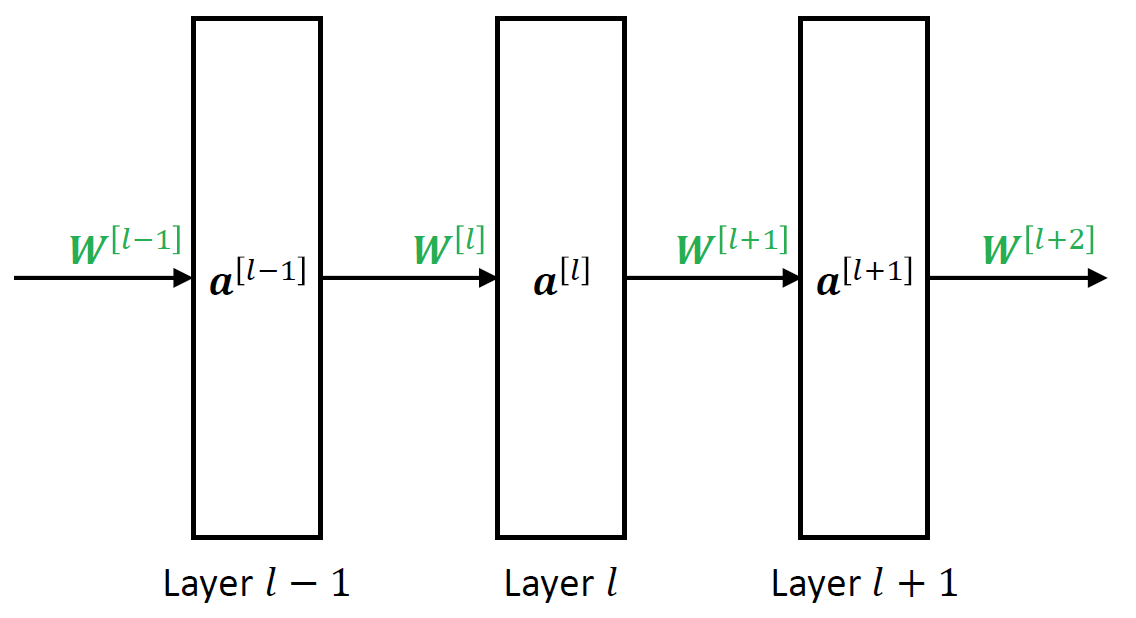
\includegraphics[width=0.5\linewidth]{neural-network}
		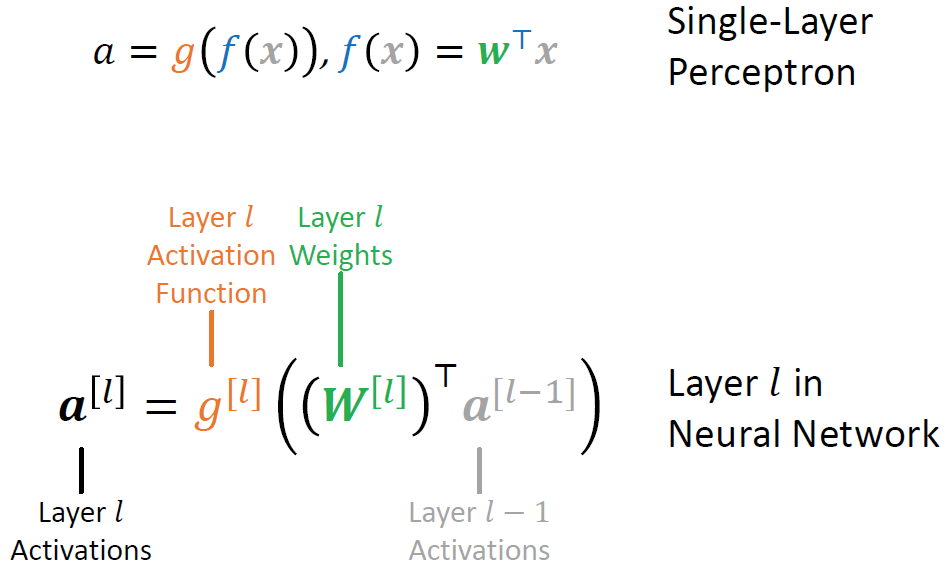
\includegraphics[width=0.5\linewidth]{layer-activation}
	\end{tabular}
	\subsubsection{Single-output Neural Network}
	\begin{center}
		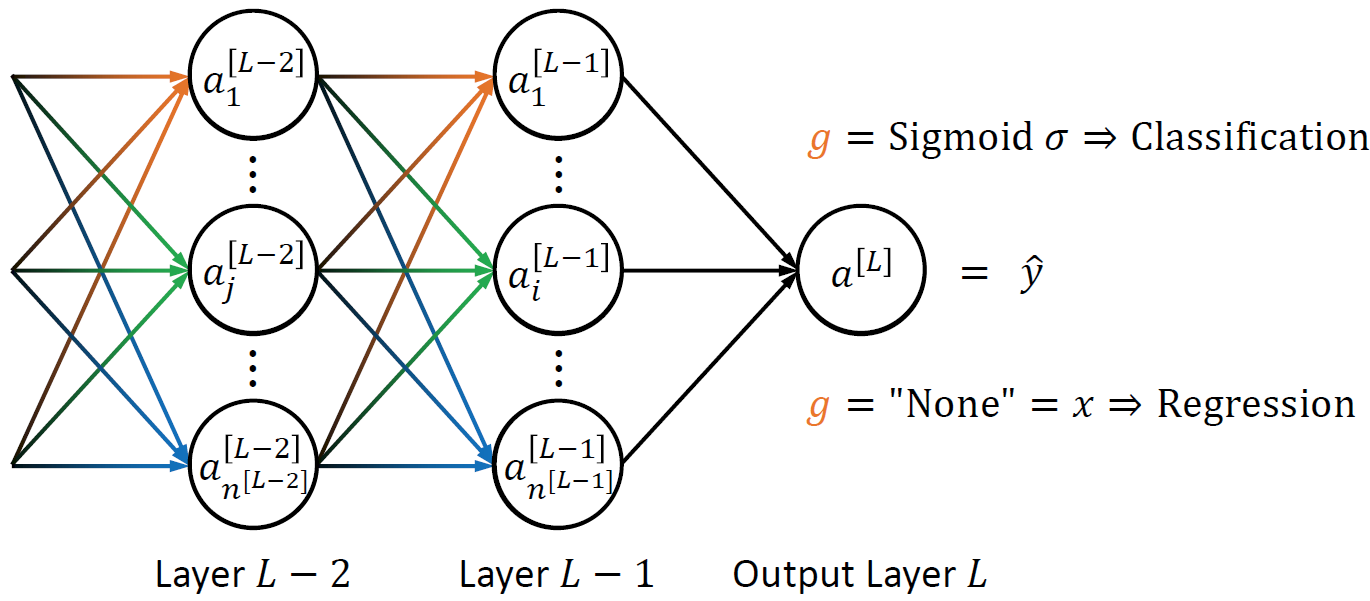
\includegraphics[width=0.7\columnwidth]{single-neural-net}
	\end{center}
	\subsubsection{Multi-class Neural Network}
	Error $\varepsilon=-y\cdot\log\hat{y}$
	\begin{center}
		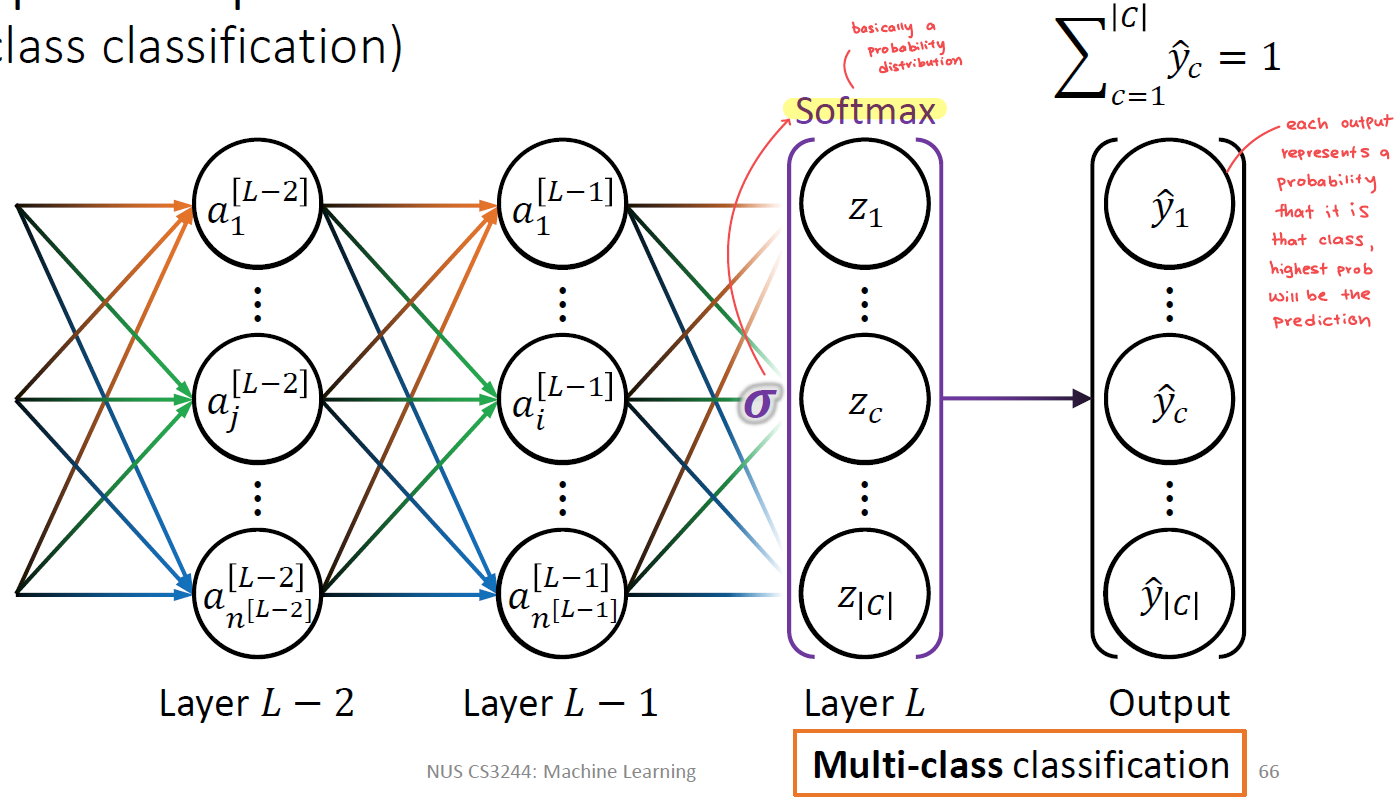
\includegraphics[width=0.6\columnwidth]{multi-class}
	\end{center}
	\subsubsection{Multi-label Neural Network}
	Error $\varepsilon=||y-\hat{y}||^2$
	\begin{center}
		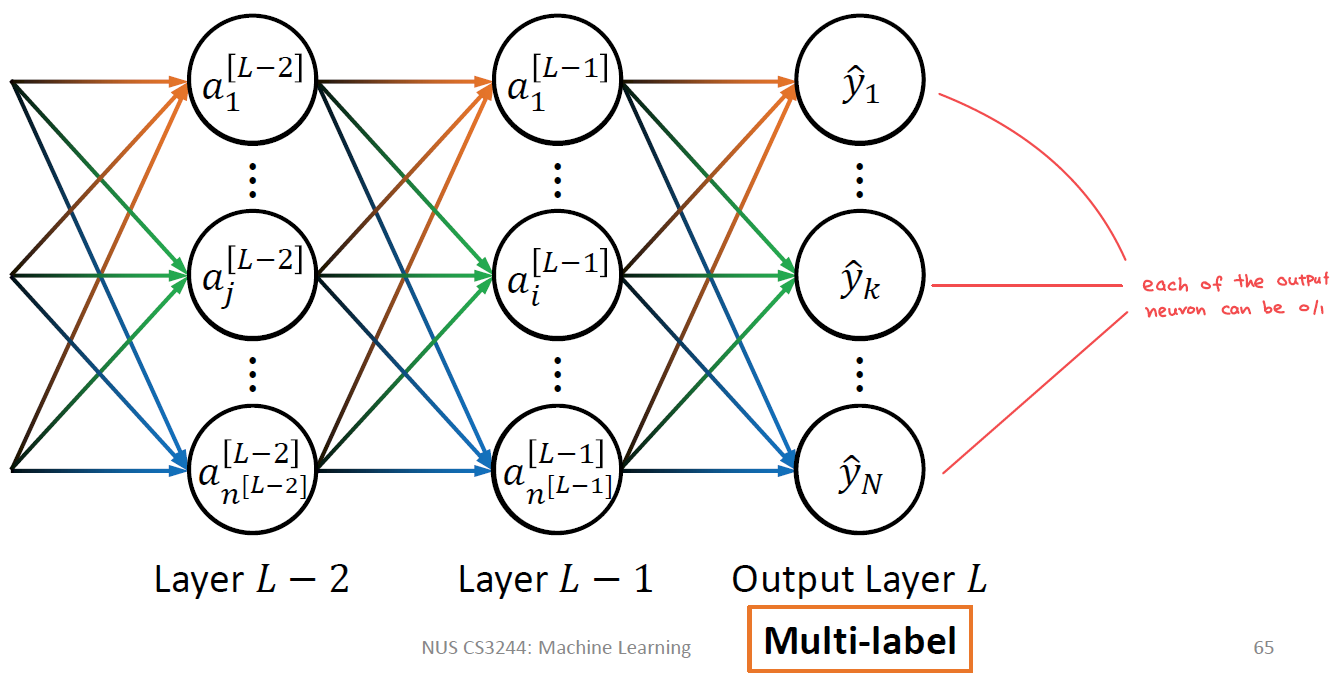
\includegraphics[width=0.6\columnwidth]{multi-label}
	\end{center}
	\subsubsection{Sigmoid vs Softmax}
	\begin{center}
		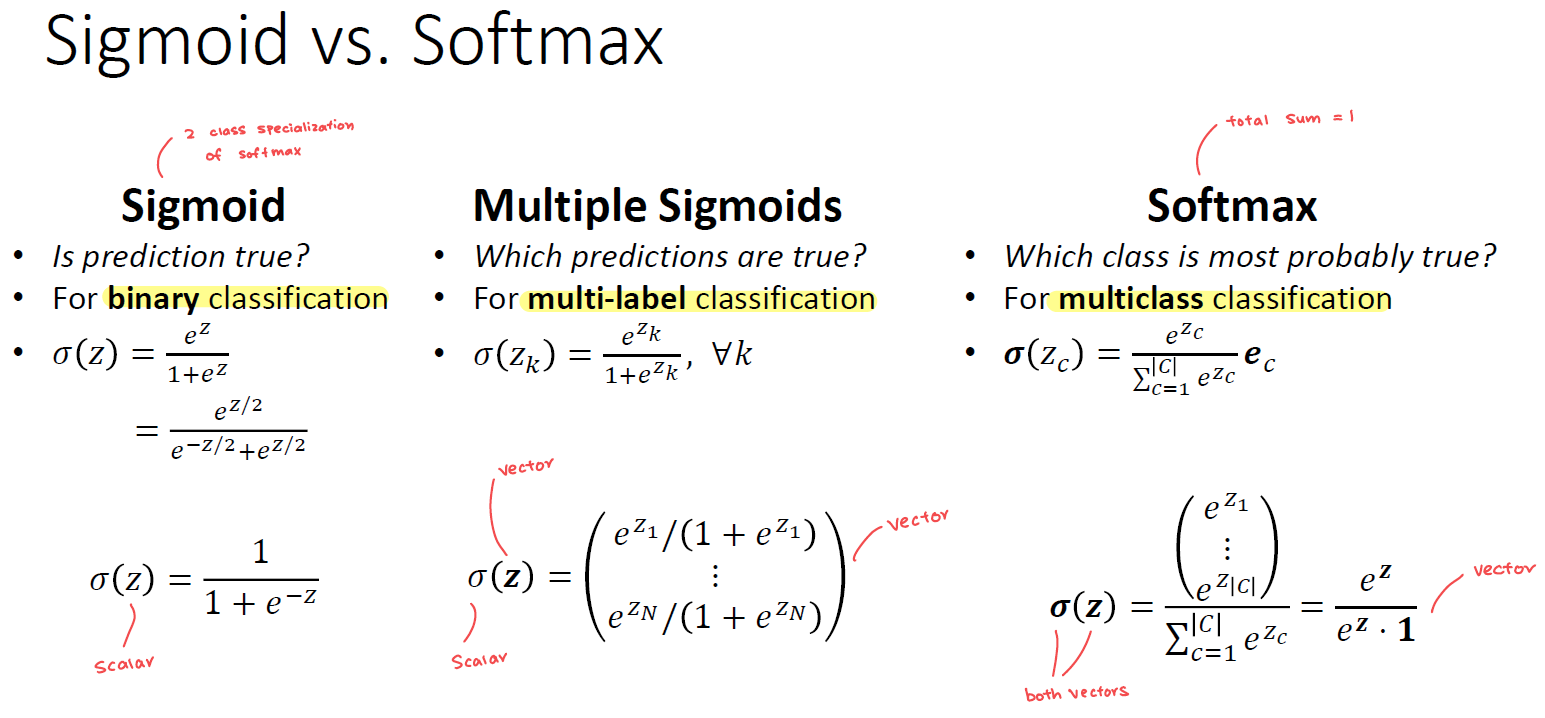
\includegraphics[width=0.6\columnwidth]{sigmoid-vs-softmax}
	\end{center}
	\section{Backpropagation}
	\subsection{What is Backpropagation}
	\begin{itemize}
		\item Used to \textbf{efficiently} compute the \textbf{gradient of the weighted input of each layer} from the last layer of the neural network to the front
		\begin{itemize}
			\item avoids duplicate calculation
			\item doesn't compute unnecessary intermediate values
			\item computes gradient of each layer
		\end{itemize}
		\item Idea for backpropagation is that the error of the prediction is propagated backwards through network, leading to adjustment of the weights and biases to minimize error
		\item Backprop relies on the fact that each \textcolor{red}{function/layer is differentiable}
	\end{itemize}
	\begin{center}
		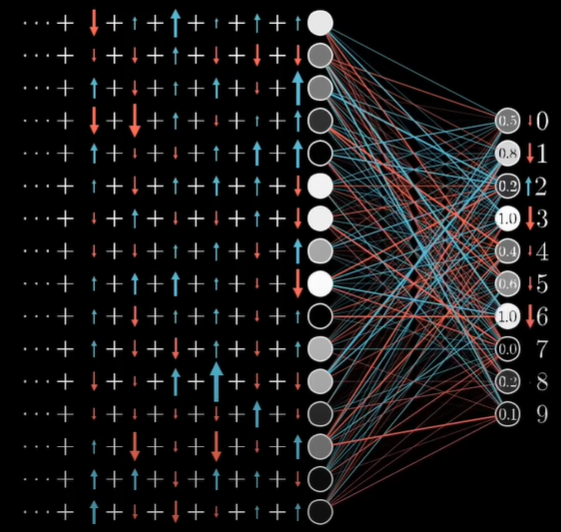
\includegraphics[width=0.5\columnwidth]{backprop-visualization}
	\end{center}
	\subsection{Important Math Notations}
	\[\frac{d\hat{y}}{d\textbf{W}^{[l]}}=\boldsymbol{a}^{[l-1]}(\boldsymbol{\delta}^{[l]})^T\]
	\[\boldsymbol{\delta}^{[l]}=\left(\frac{dg^{[l]}}{df^{[l]}}\right)(\textbf{W}^{[l+1]}\boldsymbol{\delta}^{[l+1]})\]
	\[\frac{d\varepsilon}{d\boldsymbol{W}^{[l]}}=\frac{d\varepsilon}{d\hat{y}}\frac{d\hat{y}}{d\boldsymbol{W}^{[l]}}\]
	\subsection{Backpropagation Visualization}
	\begin{center}
		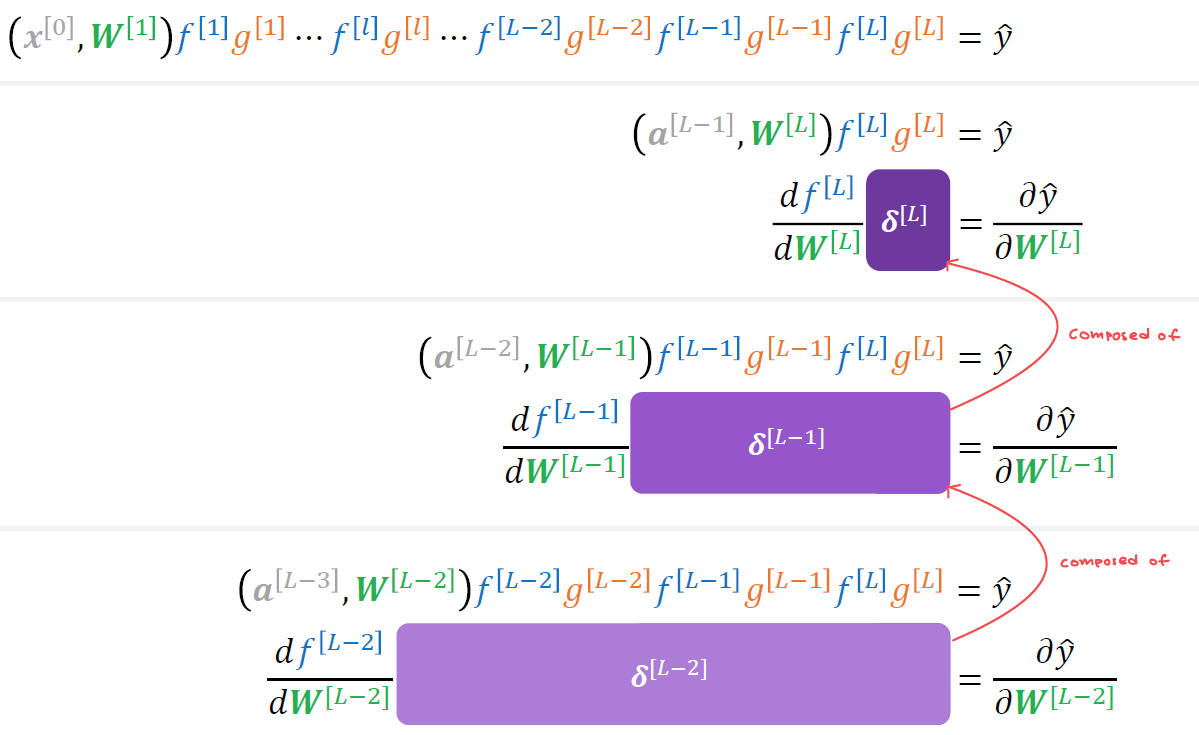
\includegraphics[width=0.7\columnwidth]{backprop}
	\end{center}
	\section{Convolutional Neural Network}
	\subsection{Deep Neural Network}
	\begin{itemize}
		\item Basically a neural net \textbf{that has $\leq 3$ hidden layers}
		\item Layerscan be convolution, pooling, concatenation, dropout, fully connected or softmax
		\item Use to \textbf{predict complex target functions} in the real world with \textbf{a lot of parameters}
		\item Requires \textcolor{red}{large amount of data} to increase performance and avoid curse of dimensionality
	\end{itemize}
	\subsection{Convolutional Neural Network}
	\begin{itemize}
		\item Suitable for \textcolor{red}{image} processing
		\begin{itemize}
			\item Image classification - detect face emotions
			\item Object detection - self-driving cars
			\item Image segmentation - cancer cell detection
		\end{itemize}
		\item Convolutionary Neural Networks layers are analogous to \textbf{applying different filters and kernels} where it gradually builds up in complexity
		\begin{itemize}
			\item First layer could be simple edge/shape detection
			\item Higher level can have more complex abstractions like shape of a tail, shape of a leg
			\item Top layer would be a general abstraction of classes that could be predicted
		\end{itemize}
	\end{itemize}
	\begin{center}
		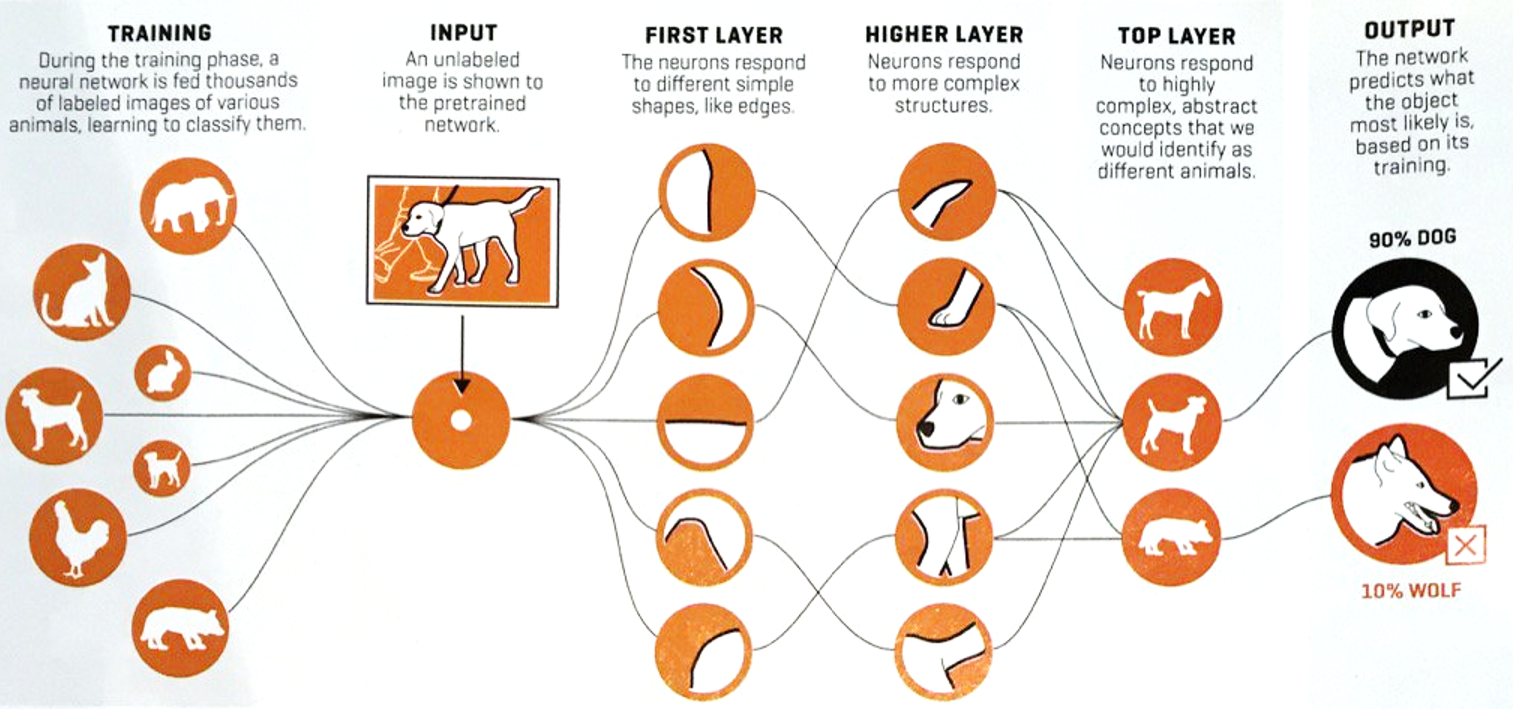
\includegraphics[width=0.6\columnwidth]{cnn}
	\end{center}
	\subsection{Kernel Size, Stride, Padding}
	\begin{minipage}{0.5\columnwidth}
		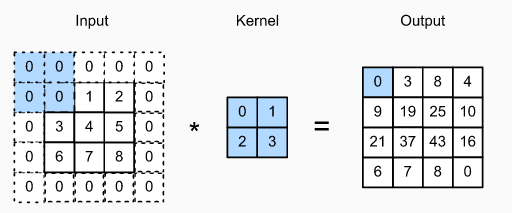
\includegraphics[width=\columnwidth]{padding}
		\captionof{figure}{Padding}
	\end{minipage}
	\hfill
	\begin{minipage}{0.5\columnwidth}
		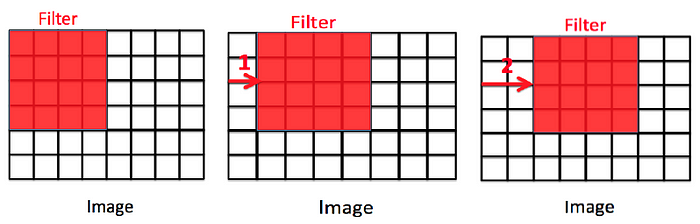
\includegraphics[width=\columnwidth]{stride}
		\captionof{figure}{Stride}
	\end{minipage}
	\subsubsection{Calculation for Output Dimension}
	\[\text{dim}\boldsymbol{y}=\left\{\left(\left\lfloor\frac{h_x+h_p-h_k}{h_s}\right\rfloor+1\right)\times\left(\left\lfloor\frac{w_x+w_p-w_k}{w_s}\right\rfloor+1\right)\right\}\]
	\begin{itemize}
		\item $h_x,w_x$ is the row x col of the input
		\item $h_p,w_p$ is row x col of padding
		\item $h_k,w_k$ is row x col of kernel
		\item $h_s,w_s$ is row x col of stride
	\end{itemize}
	\subsection{Multi-Channel Convolution}
	\begin{itemize}
		\item Have 1 kernel for each channel (R, G, B) of the image, do convolution and then add up the resulting 2d matrix
	\end{itemize}
	\begin{center}
		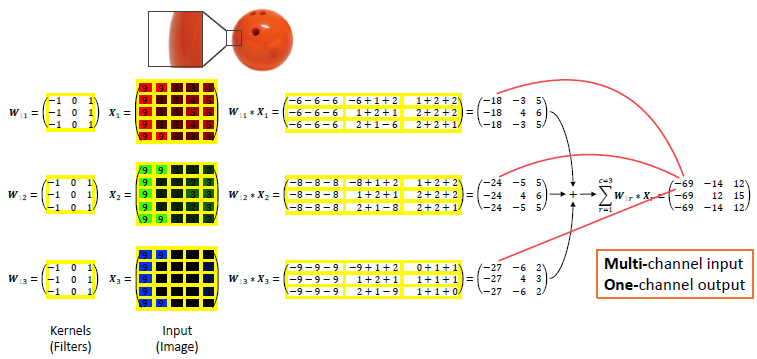
\includegraphics[width=0.65\columnwidth]{multi-channel-convolution}
	\end{center}
	\subsection{Multiple Convolution Kernels}
	\begin{itemize}
		\item Each kernel now convolves on \textbf{all channels} of the image
		\item Can think of \textbf{each kernel looking for specific "feature"} of the image (e.g. which part was more yellow, pink, orange etc.)
		\item Results in an \textbf{activation map} that basically tells you which part of the image each feature lies more in
		\item Concat the activation maps together in final output
	\end{itemize}
	\begin{center}
		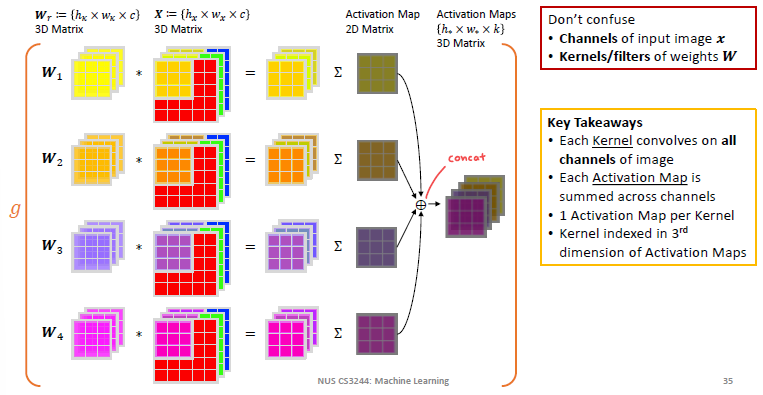
\includegraphics[width=0.6\columnwidth]{multi-convolution-kernels}
	\end{center}
	\subsection{Multi-Channel Multi-Kernel Convolution}
	\begin{minipage}{0.3\columnwidth}
		\begin{center}
			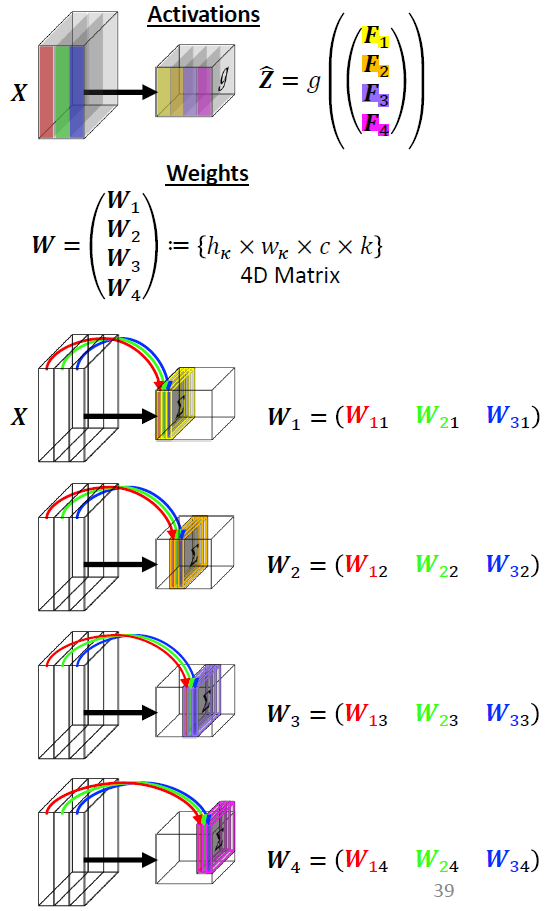
\includegraphics[width=1\columnwidth]{mcmk-conv}
		\end{center}
	\end{minipage}
	\begin{minipage}{0.6\columnwidth}
		\begin{itemize}
			\item Intuition is that multi-channel is used to detect color-specific features whereas multi-kernel can be used to detect different kinds of features (e.g. edges, textures etc.)
			\item In a multi-channel multi-kernel convolution operation, \textbf{each kernel is applied to the corresponding channel} of the input data, and the results are summed to produce the final output feature map. This process allows the network to \textbf{detect complex patterns} in the input data by \textbf{combining the features detected by the different kernels}
		\end{itemize}
	\end{minipage}
	\subsection{Fully Connected vs Convolution Layers}
	\begin{tabular}{c c}
		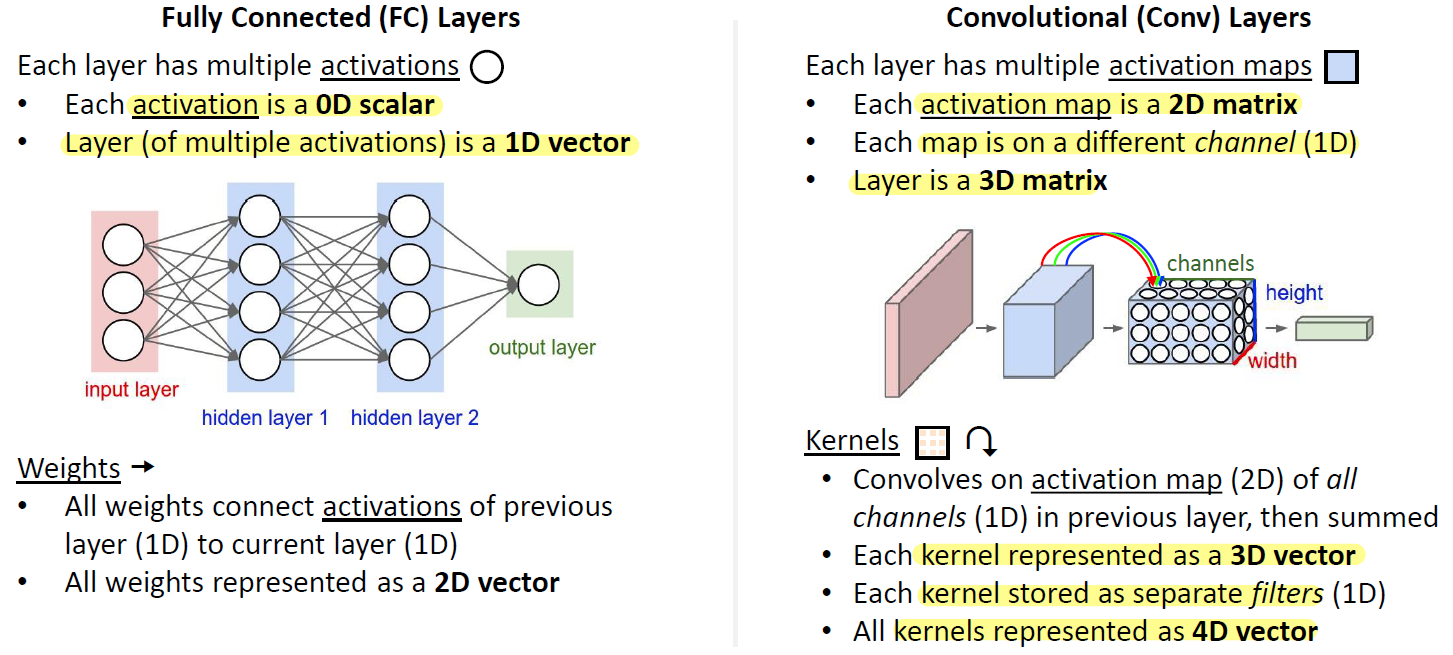
\includegraphics[width=0.5\linewidth]{fc-vs-conv-layers}
		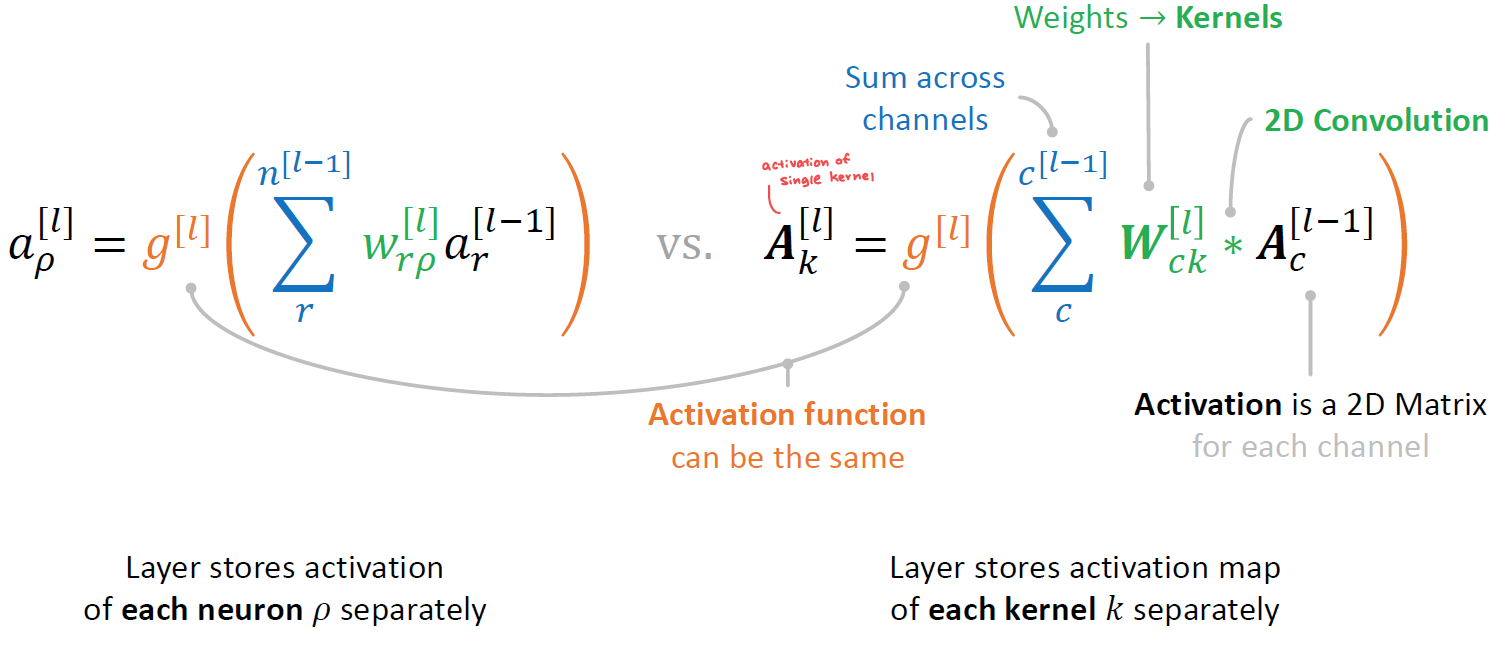
\includegraphics[width=0.5\linewidth]{fc-vs-conv-layers-2}
	\end{tabular}
	\subsection{Convolutional Layers}
	\begin{itemize}
		\item Typically \textbf{starts off with relatively low number of kernels} to detect basic features, \textbf{increase number of kernels in deeper layers} to get \textbf{more descriptive power} as we combine more and more simple features
	\end{itemize}
	\begin{center}
		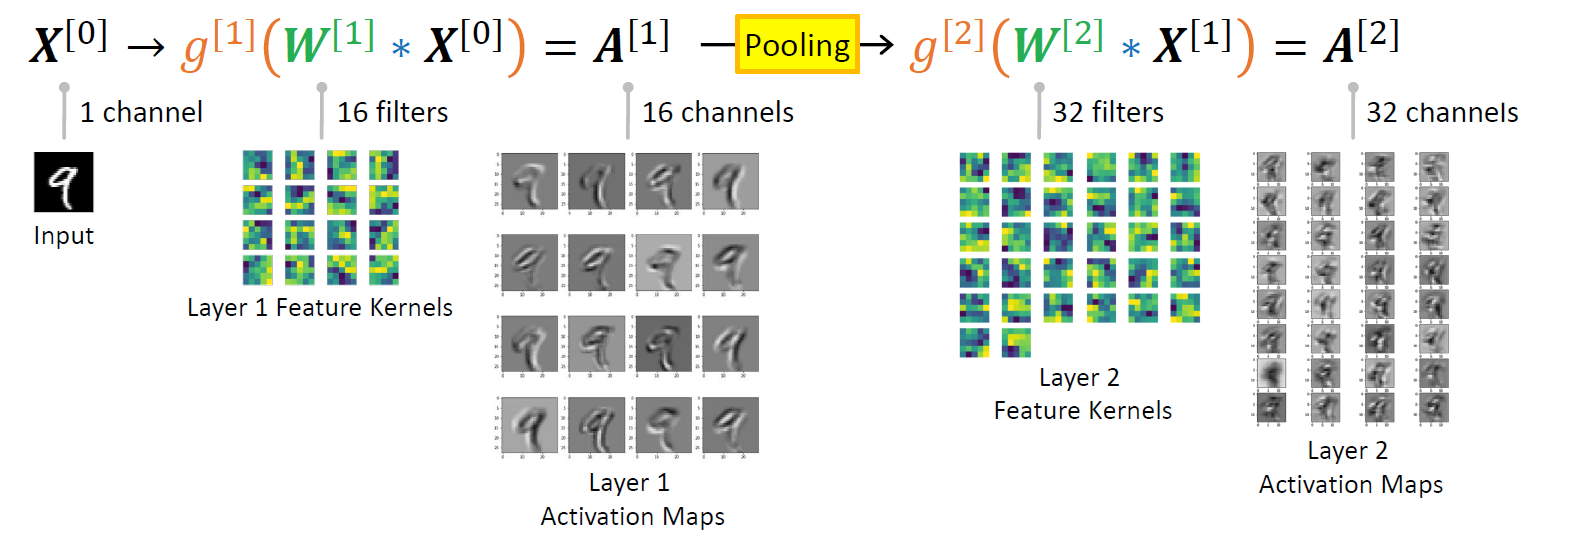
\includegraphics[width=0.6\columnwidth]{conv-layer}
	\end{center}
	\begin{itemize}
		\item Uses \textbf{pooling} layers to \textbf{downsample} feature maps which helps to train later kernels to detect \textbf{higher-level} features
		\item Also helps in \textbf{reducing dimensionality}
		\item Typical methods are max-pool (most common), average pool, sum-pool
	\end{itemize}
	\begin{center}
		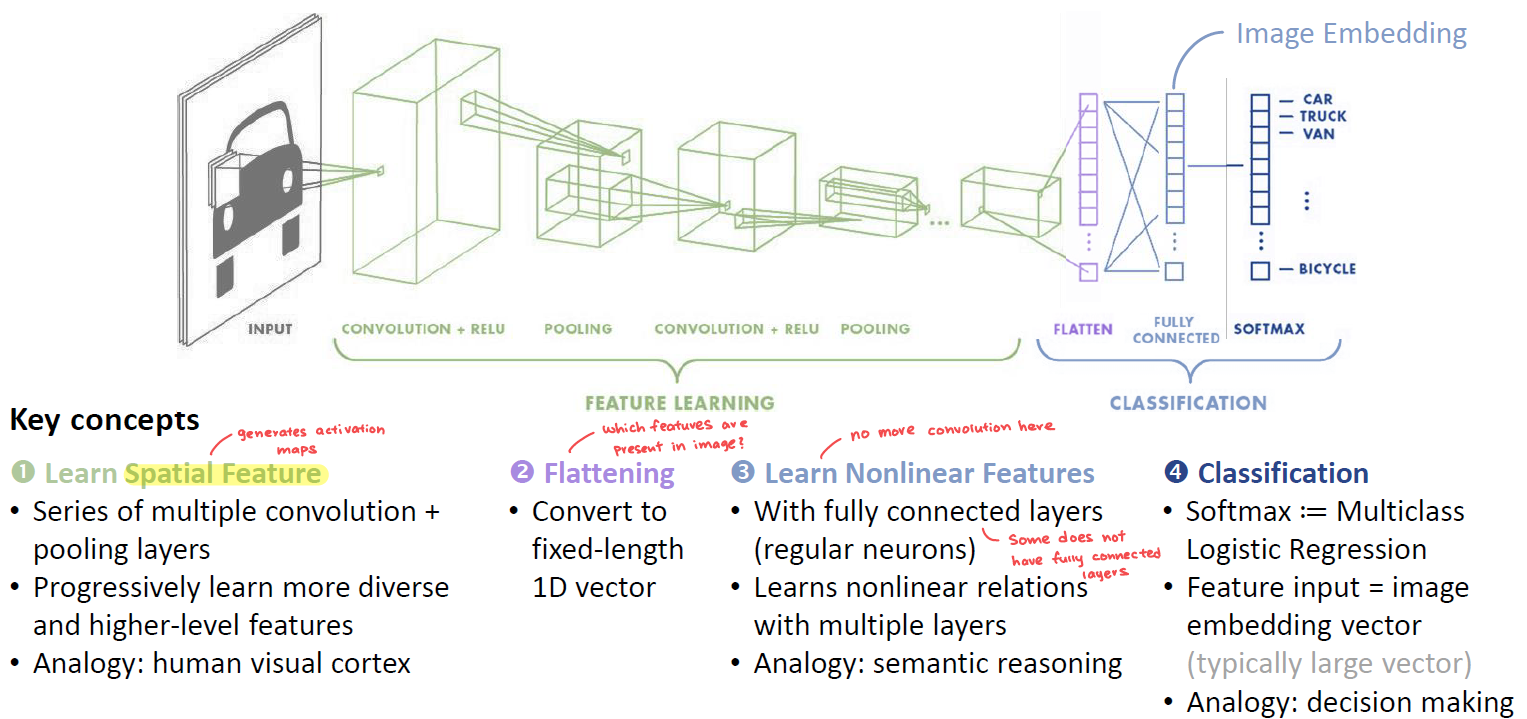
\includegraphics[width=0.65\columnwidth]{cnn-layers}
	\end{center}
	\columnbreak
	\section{Recurrent Neural Network}
	\begin{itemize}
		\item Suitable for \textbf{text} and \textbf{time series} data
		\item Used in applications like speech recognition, music generation, sentiment classification, DNA sequence analysis, machine translation
		\item Output of the hidden layers of the \textbf{previous time step} is fed into the training of the hidden layer of the \textbf{next time step}
		\begin{itemize}
			\item Notion of \textbf{using past data to predict things in the future}
			\item We are using the output of the hidden layer of the previous time step and not just the input data of the previous time step as hidden layer contains a \textbf{more "compressed" representation} of the input data with \textbf{mostly useful information}
		\end{itemize}
		\item Weights for training each time step \textcolor{red}{remains the same} for \textbf{efficiency} and to ensure that model can \textbf{predict independent of time}
	\end{itemize}
	\[\boldsymbol{\hat{y}}_t=g^{[y]}(\boldsymbol{h}_t)\]
	\[\boldsymbol{h}_t=g^{[h]}(\boldsymbol{x}_t,\boldsymbol{h}_{t-1})\]
	\begin{tabular}{c c}
		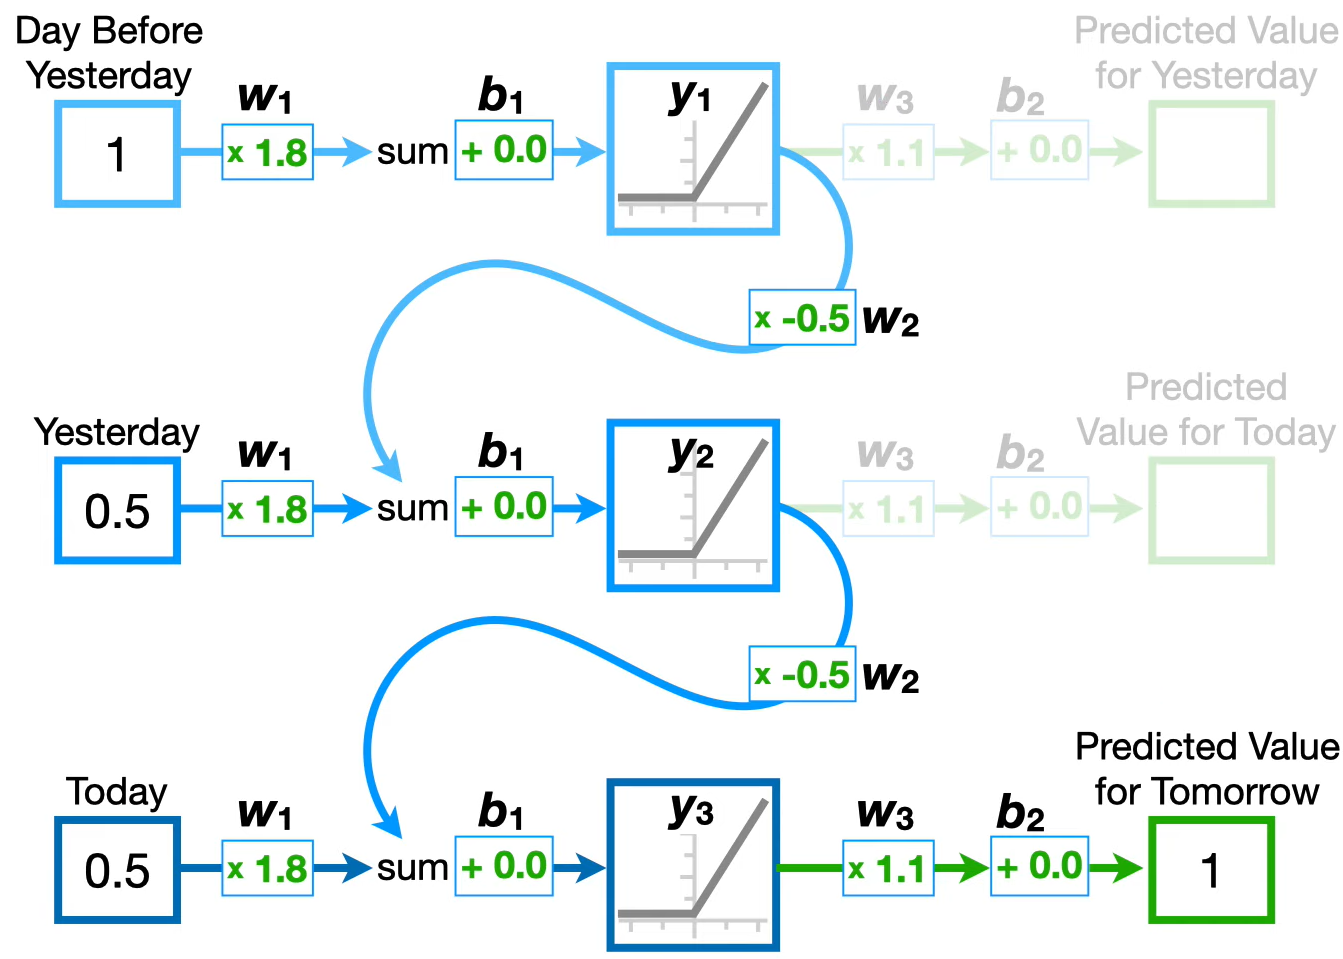
\includegraphics[width=0.45\linewidth]{rnn}
		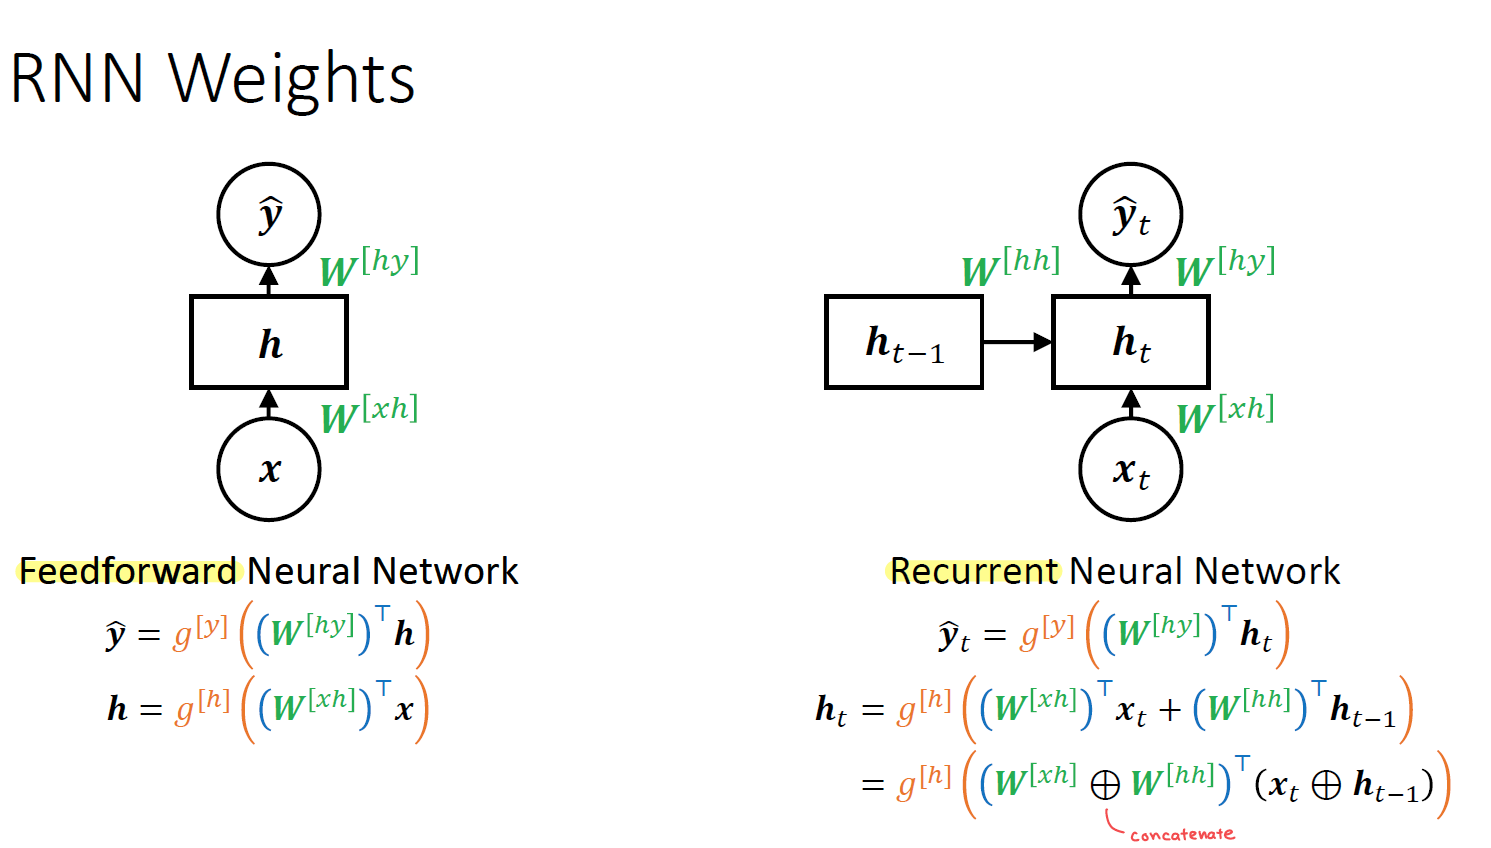
\includegraphics[width=0.55\linewidth]{rnn-weights}
	\end{tabular}
	\subsection{Backpropagation Through Time}
	\begin{center}
		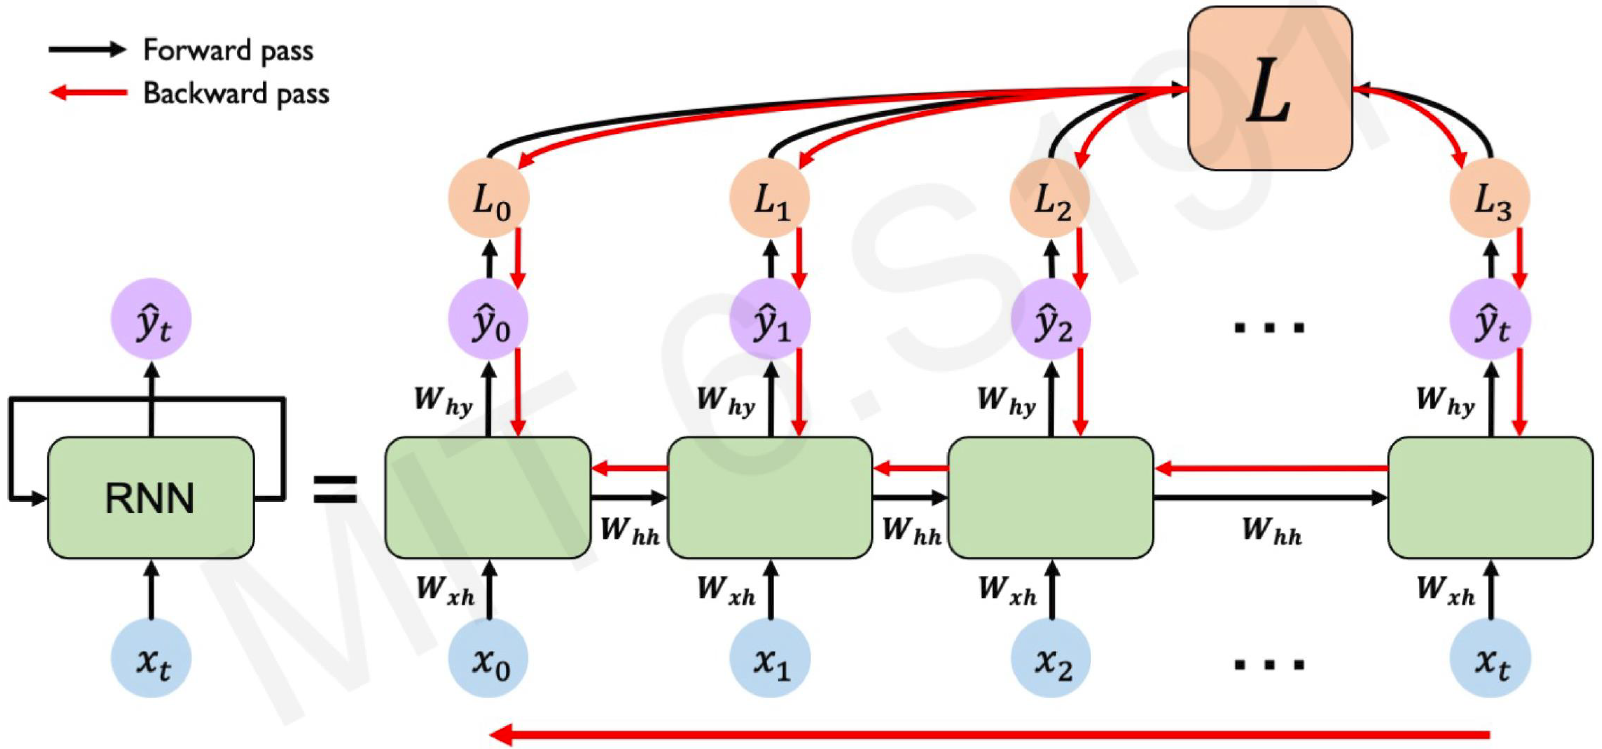
\includegraphics[width=0.7\columnwidth]{backprop-through-time}
	\end{center}
	\begin{itemize}
		\item In typical feed-forward neural nets, the backpropagation only occurs through \textbf{one of the verticals in the diagram}
		\item However, in RNN, since there is a notion of time data, we also have to propagate the weight information through the \textbf{horizontal (time) axis}
		\item \textbf{Extremely slow} since we have to complete the entire sequence for all the time steps before we can do any gradient/weight updates
		\begin{itemize}
			\item \textbf{Transformers} are a way to speed them up by calculating the backprop in parallel without needing to depend on the next time step
		\end{itemize}
	\end{itemize}
	\subsection{Training RNN vs Prediction using RNN}
	\begin{tabular}{c c}
		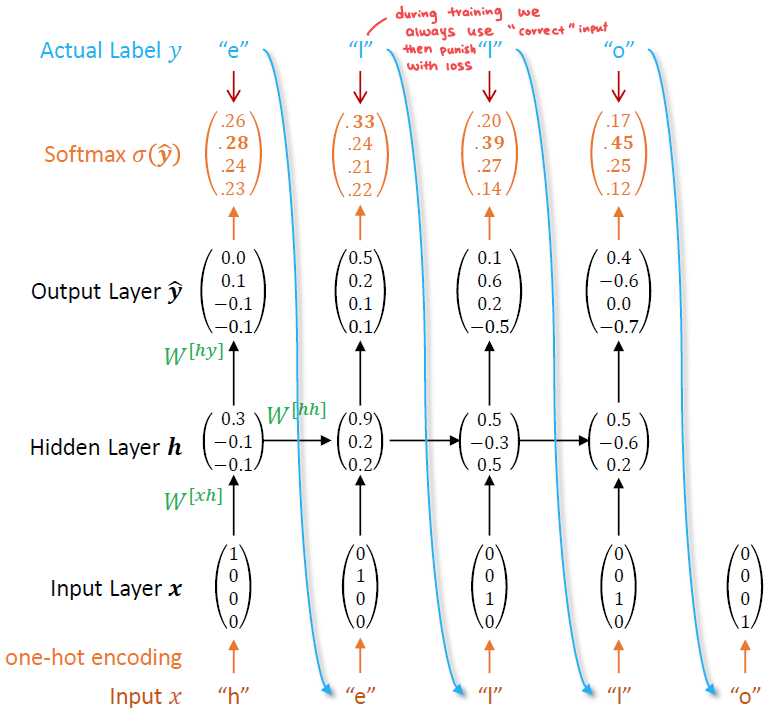
\includegraphics[width=0.5\linewidth]{training-rnn}
		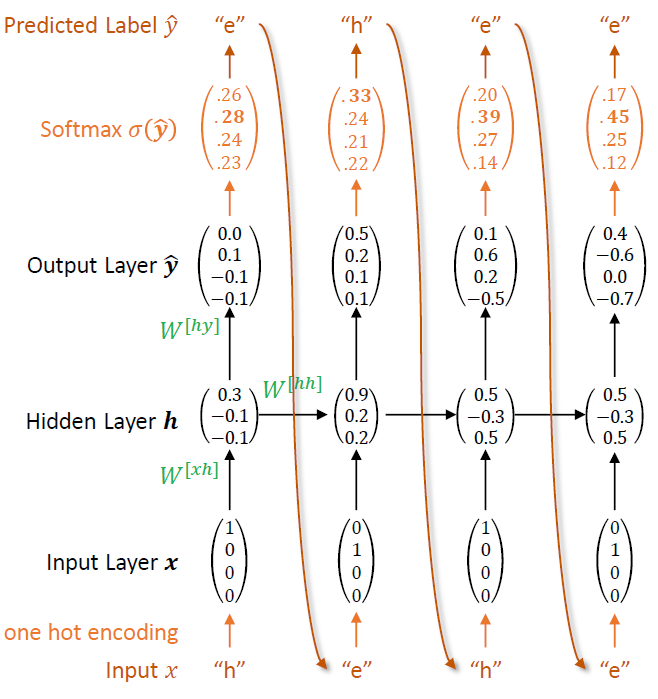
\includegraphics[width=0.5\linewidth]{rnn-predict}
	\end{tabular}
	\begin{itemize}
		\item During training, we will always want to feed in the \textbf{actual label as input} for each of the time step
		\item During prediction, the input of the next timestep will be the \textbf{predicted label} in the previous timestep
	\end{itemize}
	\subsection{Types of Sequence Modeling}
	\begin{center}
		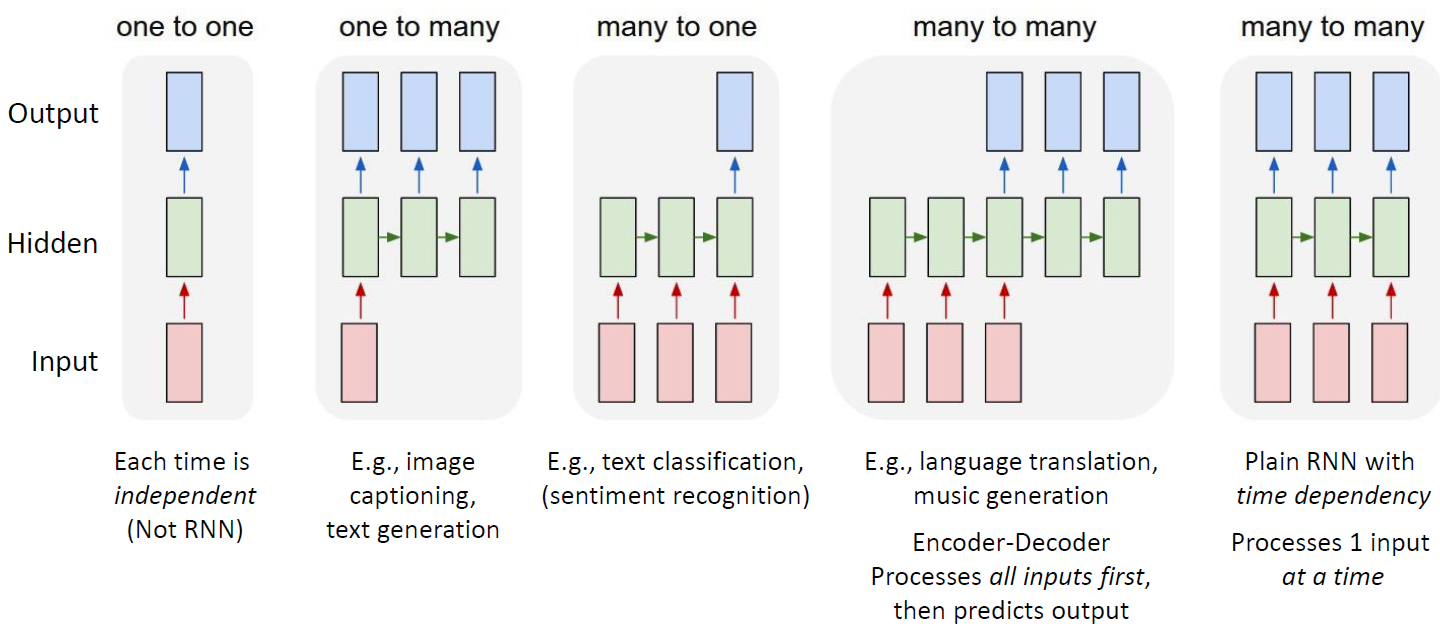
\includegraphics[width=0.7\columnwidth]{types-of-modeling}
	\end{center}
	\subsection{RNN Training Issues}
	\subsubsection{Overfitting}
	\begin{itemize}
		\item Recap: overfitting is when the performance of validation < training
		\item RNN/Deep Learning models can overfit when there are \textbf{too many parameters} and model is \textbf{more expressive than needed}
		\item Mitigation:
		\begin{itemize}
			\item Gather more data and get larger training dataset
			\item Implement a \textbf{dropout} layer - \textbf{randomly drop out} neurons during batch training so that you \textbf{disallow propagation} through these neurons
			\begin{itemize}
				\item Note that \textbf{all neurons still used for prediction}
			\end{itemize}
		\end{itemize}
	\end{itemize}
	\subsubsection{Saturating/Vanishing Gradient Problem}
	\begin{tabular}{c c}
		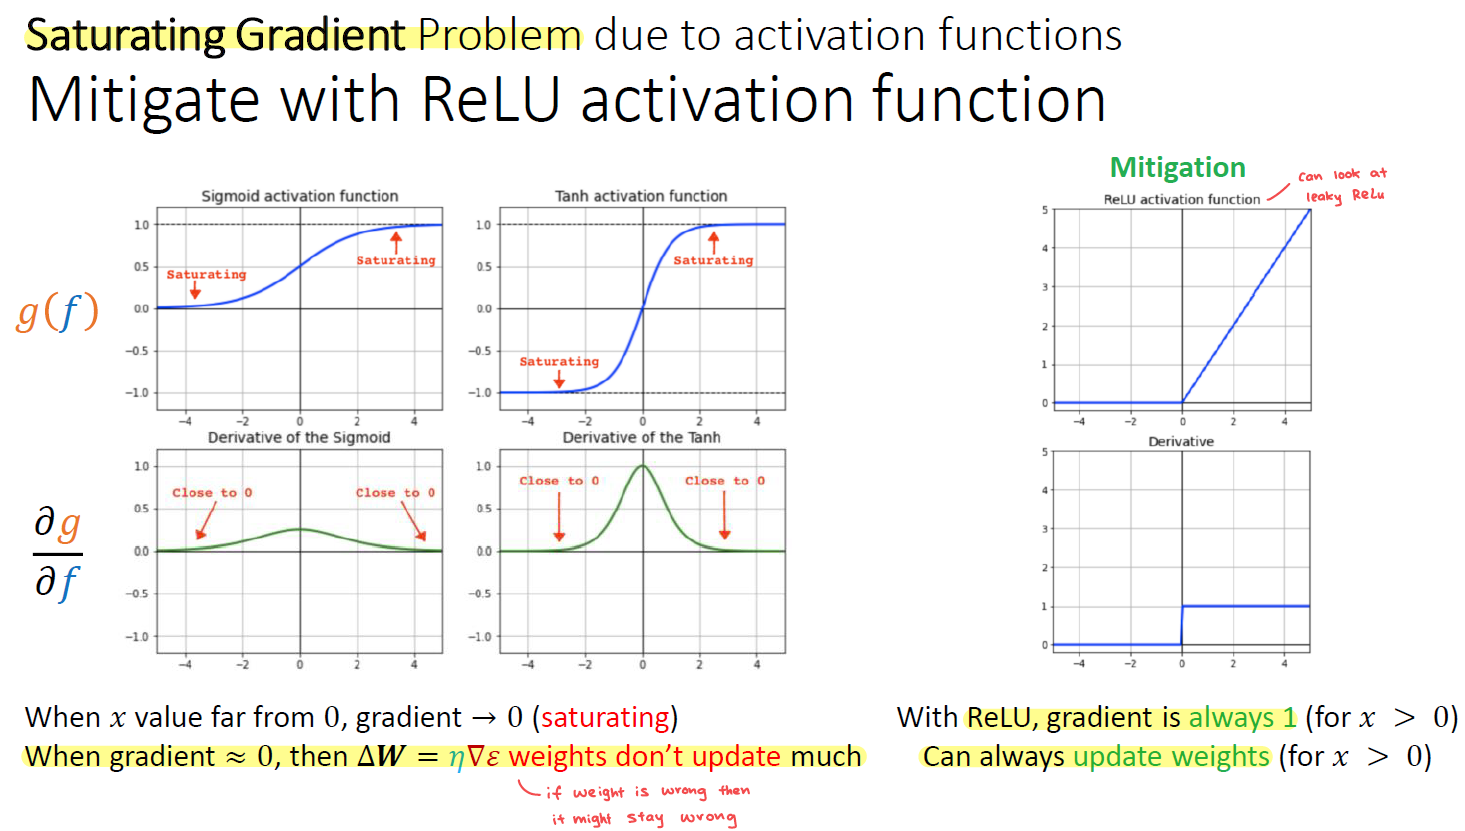
\includegraphics[width=0.5\linewidth]{saturating-gradient}
		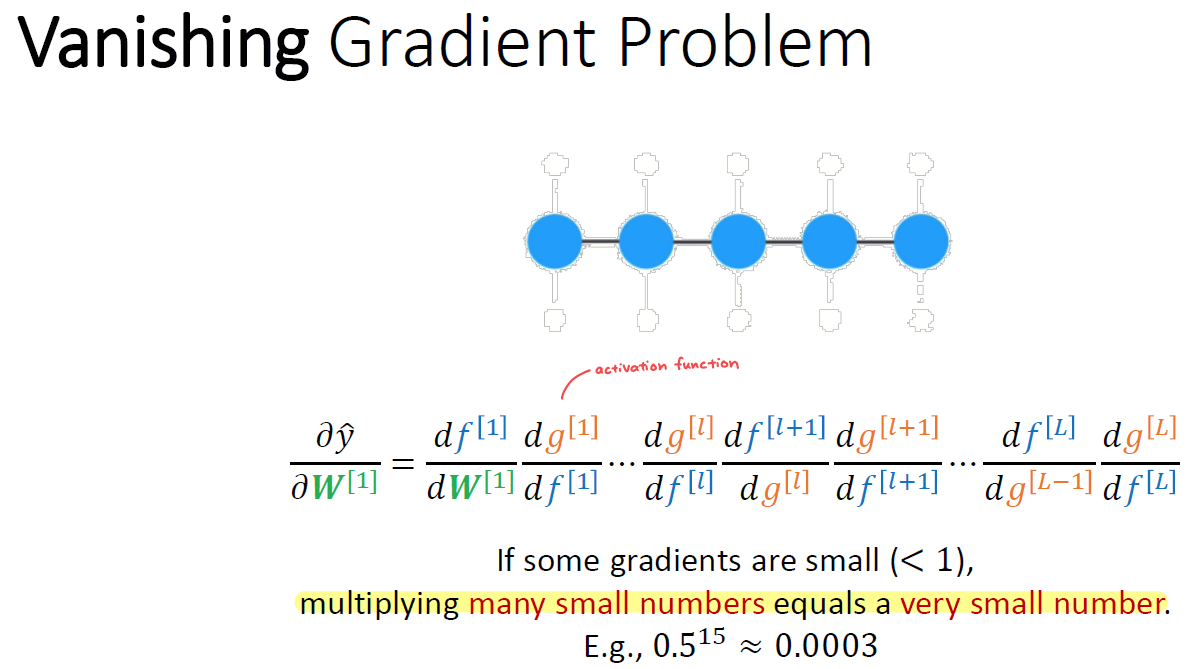
\includegraphics[width=0.5\linewidth]{vanishing-gradient}
	\end{tabular}
	\section{Explainable AI (XAI)}
	\subsection{Feature Importance}
	\begin{itemize}
		\item Want to explain what features are \textbf{important} for prediction and in what ways the features \textbf{influenced} the prediction
		\item Implementations:
		\begin{enumerate}
			\item \textbf{Weights} for linear/logistic regression
			\item \textbf{Surrogate Weights} from LIME 
			\item \textbf{Saliency Maps} (heatmap) of CNN
		\end{enumerate}
	\end{itemize}
	\subsection{Intepreting Logistic and Linear Regression}
	\begin{minipage}{0.5\columnwidth}
		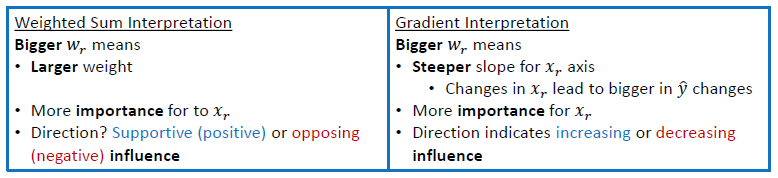
\includegraphics[width=\columnwidth]{xai-linear}
		\captionof{figure}{Linear Regression}
	\end{minipage}
	\hfill
	\begin{minipage}{0.5\columnwidth}
		\includegraphics[width=\columnwidth]{xai-logistic}
		\captionof{figure}{Logistic Regression}
	\end{minipage}
	\subsection{Local Interpretable Model-Agnostic Explanations (LIME)}
	\subsubsection{Naive Approaches to Describe Non-linear Decision Boundary}
	\begin{enumerate}
		\item Use \textbf{linear model} to explain a complicated non-linear model
		\begin{itemize}
			\item Simple to interpret
			\item Too much error between explanation function and actual prediction function - lots of false positives and false negatives if we use simple linear model
		\end{itemize}
		\item Use gradients to explain non-linear model
		\begin{itemize}
			\item Calculates steepness for each feature $x_r$
			\item \textcolor{red}{Difficult to remember}, since gradients are different for each instance (point)
		\end{itemize}
	\end{enumerate}
	\subsubsection{LIME}
	\begin{minipage}{0.5\columnwidth}
		\begin{center}
			\includegraphics[width=1\columnwidth]{lime}
		\end{center}
	\end{minipage}
	\begin{minipage}{0.5\columnwidth}
		\begin{enumerate}
			\item Choose an instance $\boldsymbol{x}$ to explain
			\item Focus on a \textcolor{red}{local} region
			\item Get training set as the neighbors of $\boldsymbol{x}$
			\item Train a surrogate \textbf{linear} model $g(x)=w\cdot x=\sum_{r=0}^{n}w_rx_r$, where the weights are higher the closer they are to $x$
		\end{enumerate}
	\end{minipage}
	\begin{center}
		\includegraphics[width=0.6\columnwidth]{lime-math}
	\end{center}
	\begin{itemize}
		\item Model-agnostic means that LIME can be \textcolor{red}{used for explaining any models}
		\item Note that it only gives explanation for a local area
		\begin{itemize}
			\item If area is defined big enough then can explain "globally"
		\end{itemize}
	\end{itemize}
	\subsection{Gradient-Weighted Class Activation Mapping (GRAD-CAM)}
	\begin{itemize}
		\item Used when explaining \textbf{images} as it has \textbf{too many features} which is unsuitable for LIME
		\item Explains using something called \textbf{saliency map} which is basically a heat map
		\item Grad-CAM aims to apply to idea of feature importance to activation maps
	\end{itemize}
	\begin{center}
		\includegraphics[width=0.7\columnwidth]{grad-cam}
	\end{center}
	\section{Unsupervised Learning}
	\subsection{K-Means Clustering}
	\subsubsection{Clustering Applications}
	\begin{itemize}
		\item Customer segmentation, Image Segmentation, Behavior Segmentation, Color Quantization (reduce image size)
	\end{itemize}
	\subsubsection{Intuition of K-Means}
	\begin{minipage}{0.5\columnwidth}
		\begin{center}
			\includegraphics[width=1\columnwidth]{k-means}
		\end{center}
	\end{minipage}
	\begin{minipage}{0.5\columnwidth}
		\begin{itemize}
			\item Group clusters and try to \textbf{minimize} within-cluster variance
			\item More variance $\rightarrow$ more dissimilaraity between members of the same cluster
			\item Metric for variance is \textbf{Within-Cluster Sum-of-Squares} (WCSS) $L$: $$\underset{s}{\mathrm{argmin}}\sum_{c=1}^{k}\sum_{x\in S_c}||x-\mu_c||^2$$
			\item WCSS is the sum of the squared distances between each data point in a cluster and its centroid. It's calculated for each cluster and then summed up for all clusters.
		\end{itemize}
	\end{minipage}
	\subsubsection{k-means Clustering Algorithm}
	\begin{center}
		\includegraphics[width=0.7\columnwidth]{k-means-algo}
	\end{center}
	\subsubsection{Elbow Method}
	\begin{minipage}{0.4\columnwidth}
		\begin{center}
			\includegraphics[width=1\columnwidth]{elbow-method}
		\end{center}
	\end{minipage}
	\begin{minipage}{0.5\columnwidth}
		\begin{itemize}
			\item Used to determine $\boldsymbol{k}$ (number of clusters)
			\item $k$ increases with diminishing returns $\rightarrow$ when $k$ is too high, there is a marginal decrease in WCSS
			\item Ideal $k$ is the points just before the marginal returns starts
		\end{itemize}
	\end{minipage}
	\subsubsection{k-means VS kNN}
	\begin{center}
		\includegraphics[width=0.7\columnwidth]{kmeans-vs-knn}
	\end{center}
	\subsection{Autoencoders}
	\begin{itemize}
		\item Autoencoders are designed to efficiently \textbf{compress and encode} data
		\item Primarily used for \textbf{dimensionality reduction} or \textbf{feature learning}
	\end{itemize}
	\subsubsection{Auto-Encoder with bottleneck}
	\begin{minipage}{0.65\columnwidth}
		\begin{center}
			\includegraphics[width=1\columnwidth]{autoencoder-bottleneck}
		\end{center}
	\end{minipage}
	\begin{minipage}{0.35\columnwidth}
		\begin{itemize}
			\item Hidden layer contains a compressed representation of $\boldsymbol{x}$ which has \textbf{less redundant information}
			\item Used to \textbf{learn important features} and \textbf{reduce dimensionality}
			\item Uses the reconstruction loss function:
			\[\varepsilon_x(\hat{x},x)=(\hat{x},x)^T(\hat{x},x)\]
		\end{itemize}
	\end{minipage}
	\subsubsection{Sparse Autoencoder}
	\begin{minipage}{0.6\columnwidth}
		\begin{center}
			\includegraphics[width=1\columnwidth]{autoencoder-sparse}
		\end{center}
	\end{minipage}
	\begin{minipage}{0.4\columnwidth}
		\begin{itemize}
			\item Uses sparsity regularization to \textbf{penalize too many activations} in hidden layer
			\item Adds a L1 norm term to regular reconstruction loss function: $\lambda\left|\left|a^{[1]}\right|\right|_1$, where higher $\lambda$ means more sparse
			\item \textbf{Don't need to explicitly specify} number of neurons in bottleneck and have empirically higher performance due to it being \textbf{more flexible}
		\end{itemize}
	\end{minipage}
	\subsection{Comparison with PCA}
	\begin{itemize}
		\item Both have ability to reduce dimensionality
		\item Autoencoders with linear activation\textbf{linear activation} is similar to PCA but with non-orthogonal latent features
		\item Autoencoders performs better than PCA with \textbf{non-linear activation} since it can be more expressive
	\end{itemize}
	\subsection{How to train Autoencoders}
	\begin{itemize}
		\item Basically the same as normal neural networks using \textbf{backpropagation} with gradient descent but through \textbf{2 models} (encoder and decoder)
	\end{itemize}
	\begin{center}
		\includegraphics[width=0.7\columnwidth]{autoencoder-training}
	\end{center}
	\subsection{Applications of Autoencoder}
	\subsubsection{Feature Representation Learning}
	\begin{minipage}{0.5\columnwidth}
		\begin{center}
			\includegraphics[width=1\columnwidth]{unsup-feature-learning}
		\end{center}
	\end{minipage}
	\begin{minipage}{0.5\columnwidth}
		\begin{itemize}
			\item Basic idea is that we want to use Autoencoder to do feature learning in an \textbf{unsupervised} way to get some form of compressed latent feature representation
			\item We then freeze encoder layer and \textbf{discard decoder layer} and instead train a Fully Connected neural network using this latent representation (efficient since we training on compressed, useful information only)
			\item Benefit is that you \textbf{can train on a lot of unsupervised data} and test and tune using just a small subset of test data
		\end{itemize}
	\end{minipage}
	\subsubsection{Anomaly Detection}
	\begin{itemize}
		\item Idea is to train autoencoder which is very good at reconstruction \textbf{regular} instances
		\begin{itemize}
			\item Only train on \textbf{"good"}instances
		\end{itemize}
		\item When an irregular input comes in and autoencoder tries to reconstruct it, \textbf{error rate will be high} and we can catch it
	\end{itemize}
	\subsubsection{Denoising Autoencoder for Robust Learning}
	\begin{itemize}
		\item Idea is that you perturb dataset with noise and pass it to autoencoder to train
		\item Since autoencoders are good at removing redundant information, the goal is that autoencoder will only pick up on the non-noisy part of data and \textbf{ignore noise}
		\item Helps to get models which are \textbf{resistant and robust to noise}
	\end{itemize}
	\end{multicols*}
\end{document}